\documentclass[a4paper,12pt]{report}
\usepackage{a4wide}
\usepackage{ucs}
\usepackage[utf8x]{inputenc}
\usepackage{xcolor}
\usepackage[ czech,english]{babel}
\usepackage[pdftex, final]{graphicx}
% \usepackage[pdftex, final, colorlinks=true]{hyperref}
\usepackage{alltt}
\usepackage{paralist}
\usepackage{mdwlist}\usepackage{subfig}
\usepackage[final]{pdfpages}
\usepackage[final,pdftex, colorlinks=false]{hyperref}
\usepackage{pdfpages}
\usepackage{perpage} %the perpage package
%\MakePerPage{footnote} %the perpage package command
\usepackage{amsmath}
\usepackage{hyperref}
\usepackage{acronym}
\usepackage[font={small}]{caption}
\usepackage{multirow}


\usepackage{footmisc}

\makeatletter
\def\verbatim@font{\linespread{1}\normalfont\ttfamily}
\makeatother
%%%%%%%%%%%%%%%%%%%%%%%%%
% pro podmineny preklad
% false je defaultně


% \newif\ifbc % Pouze do bakalářské práce
%  \bctrue

%%%%%%%%%% fancy %%%%%%%%%%%
\usepackage{fancyhdr}

\fancyhead[L]{ČVUT v Praze}

\setlength{\headheight}{16pt}

% \usepackage{stdpage}


%%%%%%%%%%%% rozmery %%%%%%%%%%%%%%%%%%
\usepackage[%
%top=40mm,
%bottom=35mm,
%left=40mm,
%right=30mm
top=40mm,
bottom=35mm,
left=35mm,
right=25mm
]{geometry}


\renewcommand\baselinestretch{1.3}
\parskip=0.8ex plus 0.4ex minus 0.1 ex

%%%%%%%%%%%%%% Listings %%%%%%%%%%%%%%%%%
\usepackage[final]{listings}

\definecolor{lightGrey}{RGB}{250,250,250}
\definecolor{darkGrey}{RGB}{100,100,100}
\lstdefinelanguage{psmap}
{morekeywords={scale, mapinfo, maploc, where, end, font, fontsize, color,
border, raster, width, paper,
vpoints, vareas, vlines, symbol, size, rgbcolumn, sizecolumn, cwidth,
rotatecolumn, },
morekeywords=[2]{y, n, none},
morecomment=[l]{\#},
}
\lstdefinestyle{psmap}{
   language=psmap,
   basicstyle={\sffamily},
   keywordstyle=[1]{\bfseries},
   keywordstyle=[2]{\color{black}},
   commentstyle={\itshape},
   frame=lines,
   backgroundcolor=\color{lightGrey},
}
\lstdefinestyle{psmapInline}{
   language=psmap,
   basicstyle={\sffamily},
   keywordstyle=[1]{},
   keywordstyle=[2]{\bfseries\color{darkGrey}},
   commentstyle={\itshape},
   frame=lines,
   backgroundcolor=\color{lightGrey},
}


\lstdefinestyle{script}{
    language=bash,
    basicstyle={\ttfamily\footnotesize},
    keywordstyle={\bfseries},
    commentstyle={\itshape},
    frame=lines,
    backgroundcolor=\color{lightGrey}
}
\lstnewenvironment{psmap}[1][]
{\lstset{style=psmap,
   #1}}
   {}
\renewcommand{\lstlistingname}{Ukázka}
%%%%%%%%%%%%%%%%%%%%%%%%%%%%%%%%%

\newcommand{\klicslova}[2]{\noindent\textbf{#1: }#2}
\newcommand{\modul}[1]{\emph{#1}}
%\newcommand{\instr}[1]{\lstinline[style=psmapInline]|#1|}
\author{Matěj Krejčí}
% \pagecolor{darkGrey}
\newcommand{\necislovana}[1]{%
\phantomsection
\addcontentsline{toc}{section}{#1}
\section*{#1}
\markboth{\uppercase{#1}}{}
}


%%%%%%%%%%%%%%%%%%%%%%%%%%%%%%
\begin{document}
\pagestyle{empty}
%nastaveni velikosti footnote
\renewcommand\footnotelayout{\footnotesize}
\begin{center}
%napisy
\newcommand{\napisCVUT}{České vysoké učení technické v Praze}
\newcommand{\napisFS}{Fakulta stavební}
\newcommand{\napisObor}{Obor geoinformatika}
\newcommand{\napisKatedra}{Katedra geomatiky}
\newcommand{\napisVedouci}{Ing. Martin Landa Ph.D.}
\newcommand{\napisAutor}{Matěj Krejčí}
\newcommand{\napisDatum}{Praha 2014}
\newcommand{\napisNazevI}{Analýza a vizualizace srážkových dat }
\newcommand{\napisNazevII}{z mikrovlnných telekomunikačních spojů pomocí GIS}
\newcommand{\napisNazevAjI}{Analysis and vizualization of rainfall data from}
\newcommand{\napisNazevAjII}{microwave links using GIS}
\newcommand{\napisBakalarka}{Bakalářská práce}
\newcommand{\napisPraha}{Praha 2014}
%
% prikazy
%\newcommand{\velka}[1]{\uppercase{#1}}
\newcommand{\velka}[1]{\textsc{#1}}
%
% 
\newif\ifpatitul
\patitultrue

\ifpatitul
{\Large\velka{\napisCVUT}}\\
\velka{\Large\napisFS}\\
\vfill
{\LARGE\velka{\napisBakalarka}}
\vfill
{\large\napisPraha\hfill\napisAutor}
\newpage
\fi%patitul


{\Large\velka{\napisCVUT}}\\
{\Large\velka{\napisFS}}\\
{\Large\velka{\napisObor}}
\vfill

\includegraphics[width=3cm]{logo_cvut_cb} %~
\vfill
{\Large\velka{\napisBakalarka}}\\
{\Large\velka{\napisNazevI\\
\napisNazevII}}\\
{\large\velka{\napisNazevAjI\\
\napisNazevAjII}}
\vfill
{\large%
Vedoucí práce: \napisVedouci\\
\napisKatedra\\
\bigskip
\napisDatum\hfill\napisAutor}
\end{center}

\newpage
\definecolor{navodotisk}{RGB}{10,10,10}
\newcommand{\vlozZadani}{%
\Huge\textcolor{navodotisk}{\textsf{\textbf{ZDE VLOŽIT ORIGINÁLNÍ ZADÁNÍ}}}%
}
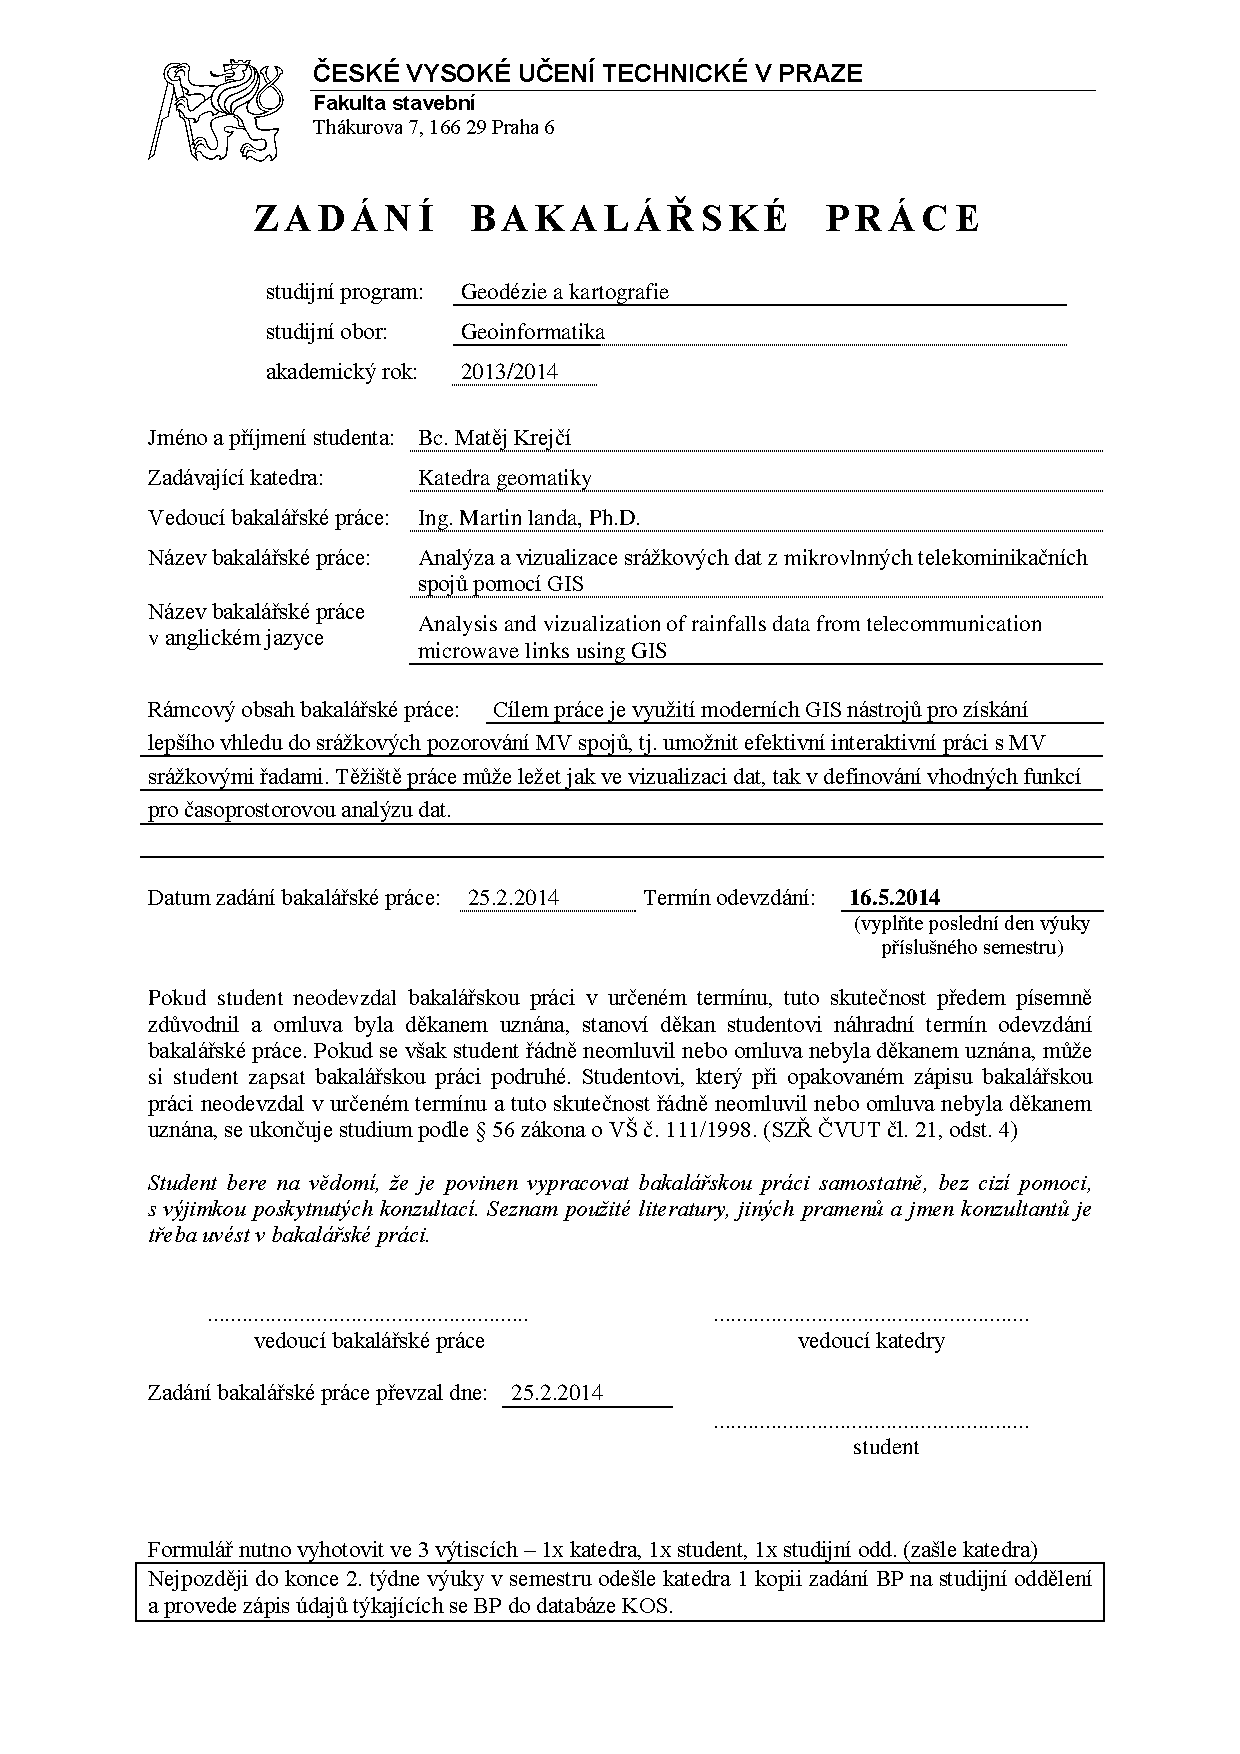
\includepdf[picturecommand={\put(100,200){\vlozZadani}}]{../formulare/zadanibp}
 % resi si zalomeni sam


\begin{abstract}
Cílem této bakalářské práce je modelování dešťových srážek z dat mikrovlnných spojů telekomunikačních operátorů. Data ke zpracování jsou uložena pomocí relační databáze PostgreSQL.
K vývoji modulu byl použit systém GRASS GIS Python API. Modul implementuje rekonstrukce dešťových srážek na základě uživatelské konfigurace. Další funkcionalitou je dávkové zpracování grafického výstupu srážek. Hlavní přínos modulu spočívá v procesu primárního zpracování dat pro následné analýzy v hydrologii a meteorologii s využitím nástroje GIS.
\bigskip

\klicslova{Klíčová slova}{GIS, GRASS GIS, Python, PostgreSQL, dešťové srážky, časoprostorová analýza, interpolace}

\end{abstract}

\selectlanguage{english}
\begin{abstract}
TODO 
\bigskip

\klicslova{Keywords}{GIS, GRASS GIS, Python, PostgreSQL, precipitation, temporal analysis,interpolation}

\end{abstract}
\selectlanguage{czech}


\newpage
\newcommand{\odsaditodzhora}{\hskip1pt\vfill}

\odsaditodzhora
\noindent Prohlášení
%%% MK: predelano po revizi
Prohlašuji, že bakalářskou práci na téma „Analýza a vizualizace srážkových dat z mikrovlnných telekomunikačních spojů pomocí GIS“ jsem vypracoval samostatně. Veškerá použitá literatura je uvedena v seznamu zdrojů.

\begin{flushleft}
\begin{tabular}{cp{0.3\textwidth}c}
V Praze dne .................
& 
&
..................................
\\
&&
(podpis autora)
\end{tabular}

\end{flushleft}
\newpage

\odsaditodzhora
\noindent Poděkování

Tady bude podekovani

\newpage

\newpage

\tableofcontents


\newpage
\necislovana{Úvod}

\pagestyle{fancy}
\setcounter{page}{1}


\subsection*{Předmluva}
Enviromentální modelování se v poslední době rozšířilo ve značném rozsahu. Velkou částí k tomu přispěla dostupnost informačních technologií a s ní spojený zájem vědeckých pracovišť o tento obor. Již ze samotného názvu vyplývá, že enviromentální modelování se zabývá životním prostředím a jeho modelováním. Pod tento obor spadá nespočetné množství podoborů, které se především liší hledáním odpovědí na rozdílné otázky. Specifikovat jednotnou definici pro enviromentálního modelování je pro jeho multidisciplinární charakter velmi obtížné. Modelování přírodních procesů vzniklo v důsledku zájmu člověka o pochopení přírody. Studium a simulace přírodních jevů a jejich zákonitostí z oborů fyzikálních, matematických, biologických, chemických v dnešní době velmi usnadňuje člověku život a v některých regionech je člověk i přímo závislý na zprostředkovaných výsledcích, které jsou produktem enviromentálních modelů. 

\subsection*{Motivace}
Modelování dešťových srážek je jednou z disciplín z oboru enviromentálního modelování. Když se poohlédneme do první poloviny 19. století, tak právě meteorologie byla jednou z prvních disciplín, která definovala pojem enviromentální modelování, tak jak ho chápeme nyní. Modelování srážek na zemském povrchu se s vývojem klimatu stává v poslední době důležitým úkolem. Oproti rozvoji fyzikálně numerických modelů a to především díky stále se zvyšujícím výpočetním výkonům počítače, nebyl technologický pokrok ve sběru srážkových dat v posledních desetiletích takřka zaznamenán. Pracovníky meteorologických a hydrologických ústavů ve vývoji brzdí nedostatečně přesná a neaktuální srážková data, která jsou jedním z hlavních vstupů pro další modely. Studie z posledních let poukazují na možnost využití mikrovlnných (MV) spojů vysílačů telekomunikačních operátorů ke sběru srážkových dat. Tento zdroj je levnější a přesnější než sběr pomocí radaru.\cite{radar_meterology} Největší potenciál sběru přesných srážkových dat v reálném čase spočívá ve vylepšení městských odtokových modelů. Pro efektivitu těchto modelů je sběr dat v dostatečném rozlišení a v reálném čase nutností.
\subsection*{Cíl}
Hlavním cílem této práce je vyvinutí nástroje pro zpracování hrubých dat z MV vysílačů v prostředí GIS, čímž se zpřístupní nespočet dalších analýz pro vývoj tohoto výzkumu. Sekundárně je práce zaměřena na využití výstupů vlastního GIS nástroje k grafické interpretaci plošných srážek. Přímo na to navazující je definování vhodných časoprostorových funkcí nástroje GIS. Téma práce bylo založeno na požadavcích zpracovatele projektu, který se zabývá problematikou odhadu srážek z MV zdrojů v rámci projektu TeleMAS v souvislosti s modelováním srážko-odtokových procesů v městských povodích. Tento projekt je řešen v úzké vědecké spolupráci s ETH-Eawag a odborné spolupráci se společnostmi T-Mobile a Veolia ČR a nyní nově s Ericsson Research (Sweden).  !!!!!Tady by měl být uveden odkaz na projekt a ten uveden v citacích!!!! 

Práce je systematicky rozdělena na část teoretickou a praktickou. V teoretické části je kladen důraz na představení základních pojmů a principů, důležitých pro část praktickou. Praktická část je charakterizována částí implementační, do které spadá vývoj vlastních GIS modulů a na část ve které je využita jejich funkcionalita společně se stávájícími nástroji GIS.

 



\newpage
\chapter{Teoretická část}
\section{Úvod do měření dešťových srážek}
První část této kapitoly má za cíl přiblížit čtenáři současné metody měření dešťových srážek. Liší se především v přesnostech, časové variabilitě a vhodností výstupu pro další využití. Tento úvod do problematiky měření srážek by měl napomoci k lepšímu pochopení výhod či nevýhod metody odhadu srážek pomocí MV, která bude v druhé části kapitoly představena a s těmito metodami porovnána. Nejdříve se ale podíváme do historie.
\subsection{Historie stručně}
Podíváme-li se do historie a opomeneme nejasné zmínky měření srážek z období 100 n.l. v Palestině, dostaneme se k přelomu 14.-15. století na území Korei za vlády krále Sejong.\cite{sejong} První náznak vynalezení srážkoměru vznikl z rozhodnutí, že místo výkopů v pudě pro kontrolu vlhkosti, bude efektivnější mít standardizovaný nástroj na měření deště. Oproti neznámým metodám měření se alespoň dochovaly zmínky o rozměrech a tvaru srážkoměru. Hlavním účelem měření bylo efektnější rozhodování panovníka při určování výše daní z obdělávaných polí farmářů. S dalším mezníkem v historii vývoje srážkoměrů měl co do činění angličan Sir Christopher Wren v letech 1661.\cite{wren} Vynalezl srážkoměr, který fungoval na principu vážení kapaliny, čímž se velmi podobal současným standardům (jeden gram vody je ekvivalentem ke krychlovému centimetru objemu vody). První měření srážek v metrických jednotkách učinil pan Benjamin Franklin. Bylo tomu v letech 1790, kdy byl poprvé metrický systém definován. Od té doby se principiálně srážkoměry nemění. Samozřejmostí je, že v průběhu staletí dochází k jejich zpřesňování přesnosti měření, standardizaci a v posledních desetiletích především k automatizaci.

Mezníkem ve sběru srážkových dat se bezesporu stal radar. Při druhé světové válce byl do provozu uveden první experimentální radar, který sloužil k metrologickému pozorování. Roku 1959 následovalo první vytvoření radarové sítě WRS-57 v USA. Postupem času se poté rozšíří metoda odhadu srážek radarem zcela globálně. \cite{flash_floods}

Nástup satelitních družic se datuje do šedesátých let 19. století. Logickou návazností na první satelitní družice vzniká obor, který dnes známe pod pojmem dálkový průzkum země (DPZ). Jedná se o zcela nový obor 20. století vyplývající z technologického pokroku. Oproti výše zmíněným metodám není DPZ zaměřen pouze pro hydrometeorologické účely. Jednotlivé družice jsou svým vybavením určeny pro měření různých veličin a jevů. Mezi historicky první meteo družice patří Vanguard 2 v roce 1959\cite{vanguard} a o rok později úspěšnější v  1960 družice TIROS-1. 
     



\subsection{Současné nástroje a metody }
\label{subsec:11}
\paragraph*{Dešťové srážky}jsou definovány jako produkt vodní páry v kapalném nebo pevném stavu a které padají z oblohy či kondenzují přímo na zemském povrchu. Srážky mohou mít formu sněhových vloček- pevné skupenství, nebo formu dešťových kapek- kapalné skupenství. Množství srážek bývá udáváno v milimetrech kapalné vody spadlé na zemský povrch za časový interval.\cite{wmo} 

\subsubsection{Srážkoměry}
Srážkoměr je přístroj používaný v meteorologii a hydrologii k měření srážkových úhrnů. Dle funkčnosti se srážkoměry dělí na dešťové a na srážkoměry, které měří i srážky pevného skupenství. Tyto srážky se přeměňují na ekvivalent vody a až pote se měří. Je zde důležité podotknout, že produktem srážkoměrů jsou bodová srážkoměrná data.


\begin{description} 
\item[Ombrometr]je jeden z nejjednodušších typů srážkoměrů. Je tvořen válcem s nálevkou, která převádí padající srážky do nádoby uvnitř válce. Srážkový úhrn se změří přelitím obsahu nádoby do kalibrovaného odměrného válce. Pro zachycení sněhu se z ombrometru sundá nálevka a sníh se nechává roztát. Tyto srážkoměry se využívají velmi zřídka.

\textbf{Výhody} jsou pouze v jednoduchosti obsluhy bez nutnosti kalibrace a také i nejmenší náklady na pořízení.
   
\textbf{Nevýhody} jsou především v nutnosti asistovaného měření. Dále pak také v nefunkčnosti přes zimní období, kdy srážkoměry zamrzají. 
\end{description}

\begin{description} 
\item[Ombrograf]se skládá z nádoby s plovákem a registračního zařízení. Srážky stékají do nádoby s plovákem, na který je napojeno registrační zařízení, které zapisuje údaj na otáčející se roli papíru. Takto vytvořený záznam se nazývá ombrogram. Záznam popisuje průběh celkového množství srážek v čase, z něho se dá odvodit intenzita srážky. Podle doby otočky bubnu kolem své osy rozlišujeme přístroje s týdenním (buben s registrační páskou se otočí o jednu otočku asi za 168 hodin) a jednodenním (otočka asi 24 hodin) chodem.\cite{chmu_navod}

\textbf{Výhody} ombrografu jsou v možnosti kontinuálního sledování srážkových úhrnů.

\textbf{Nevýhody} těchto měřících stanic jsou v přesnosti. Údaje z nich získané jsou většinou méně přesné než ze základních přístrojů. Dalším faktorem je nutnost pravidelné obsluhy, která spočívá v natažení hodinového stroje, výměny pásky a doplnění registračního inkoustu.
\end{description}

\begin{description} 
\item[Člunkový srážkoměr] je jeden z nejvíce používaných srážkoměrů současné doby. Princip jeho funkčnosti je založen na překlápěcím člunku, jehož jedna polovina se po dosažení úhrnu srážek 0.1 mm překlopí, čímž se polovina vyprázdní a začne se naplňovat druhá polovina. Takto se cyklus opakuje. Stanice překlopení zaznamenává a z počtu pulsů za určitý čas se vypočítají srážkové úhrny. Některé typy těchto srážkoměrů jsou vybaveny vyhříváním a tudíž mohou měřit i tuhé srážky.

\textbf{Výhody} těchto srážkoměrů jsou bezesporu v automatizovaném běhu stanice, bez nutných krátkodobých obsluh. 

\textbf{Nevýhody} člunkových srážkoměrů nastávají při prudkých deštích, kdy z nedostatečně rychlého překlápění člunku mohou být výsledné úhrny srážek podhodnoceny.\cite{sevruk}
\end{description}

\begin{description} 
\item[Váhový srážkoměr] funguje na principu vážení kapaliny. Váhový srážkoměr se skládá z nádoby, která je postavena na váze. Srážkoměr do nádoby zachycuje kapalinu, která je vážena tenzometrickou váhou napojenou na řídící elektronickou jednotku.

\textbf{Výhody} jsou v přesnosti měření a konstrukci srážkoměru. Tuhé srážky váhový srážkoměr zachytí a vyhodnotí bez prodlevy nutné pro jejich roztátí. Rovněž přesnost váhového srážkoměru není závislá na intenzitě srážek oproti srážkoměru s překlápěcím člunkem, kde přesnost se vzrůstající intenzitou klesá.

\textbf{Nevýhody} těchto zařízení jsou ve vyšší pořizovací ceně a díky složitosti mechanizmu představují také vyšší náklady na údržbu.
\end{description}


\subsubsection*{Chyby při měření srážkoměrem} 
Měření srážek srážkoměry jsou ovlivněny mnoha faktory, které určují konečnou přesnost a spolehlivost tohoto typu měření.
\begin{description} 
\item[Přístrojové chyby] se přesněji odvíjejí od jednotlivých zařízení. Přesnost u ombrografů se pohybuje okolo 0.2 mm do úhrnu srážek 20 mm za hodinu. Člunkové srážkoměry mají chybu měření 0.5 mm pro úhrn 20 mm srážek za hodinu. Chyby se zvyšují s vyšší intenzitou srážek. Při srážkách 150 mm za hodinu je chyba větší než 3\%. \cite{wmo}
\item[Proudění vzduchu] je jedním z nejvíce nežádoucích vlivů, které nejvýznamněji ovlivňují přesnost měření. Eliminace tohoto vlivu je velice obtížná. V nejlepším případech by mělo být zařízení ve vodorovné poloze. Z toho plynou nároky na umístění přístroje. Minimalizovat nežádoucí proudění větru se řeší pomocí několika pravidel: umístění mimo strmá území a zastavěné lokality, co nejníže k zemi, na trávník k zabránění vstupu odrážejících se kapek. Využívají se také tzv. "wind shields", které částečně chrání srážkoměry před větrem.
\item[Chyby ze smáčení] jsou způsobeny nedostatečně hydrofobním povrchem nádob a v případě srážkoměru s člunky mohou být způsobeny neúplným vylitím kapaliny při vyprazdňování. Dalším faktorem jsou přírodní vlivy, především zachycování nečistot, prachu, pavučin a dalších materiálů absorbující kapalinu. Z toho vznikají zbytkové vody, které tvoří další chyby. 
\item[Chyby z odpařování] mají vyhřívané člunkové srážkoměry. Jsou způsobeny vypařováním vody z člunku, což při malých srážkových úhrnech způsobuje značné chyby.
\item[Sklápění člunku] je hlavním problémem člunkových srážkoměrů. Při velkých deštích vstupuje voda do trychtýře i když je člunek ve stavu vylévání. To způsobuje odvádění vody, která nebyla změřena. 

\end{description}

\subsubsection{Meteorologický radar}
Radarová měření díky plošnému pokrytí a dobrému prostorovému i časovému rozlišení dat jsou vhodná pro synoptickou a leteckou meteorologii. Poskytují přehled v reálném čase o pohybu a struktuře srážkových systémů, umožňují velmi krátkodobou předpověď v řádech minut až hodin a z ní plynoucí varování před nebezpečnými meteorologickými jevy.\cite{radar_chmu}
\paragraph*{Princip}
radaru je založen na dopplerovském jevu.\cite{radar_meterology} Vysílací zařízení generuje opakovaně v řádu mikrosekund krátké elektromagnetické pulsy, které jsou vysílány ve tvaru úzkého svazku do atmosféry. Elektromagnetická energie se v atmosféře odráží jak od meteorologických objektů, tak i objektů jiných (letadla, terén). Část elektromagnetické energie, která není pohlcena nebo odražena jiným směrem, je detekována přijímačem radaru. Ze známé polohy antény, síly signálu a doby mezi jeho vysláním a přijetím se určí vzdálenost a poloha objektu, srážky. 
Pro meteorologické účely se využívá především dlouhých vlnových délek v rozsahu 1-10 cm, kterým odpovídá přibližně desetinásobek velikosti průměrných dešťových kapek nebo pevných částic. Kratších vlnových délek se využívá k zaznamenání menších částic jako je například mlha. Zde nastává problém v rychlém oslabení signálu.\cite{doppler}

\paragraph*{Srážková data}se měří obvykle v intervalu 5-15 minut. Horizontální rozlišení dat bývá 2×2 km, vertikální 1 km. Toto prostorové rozlišení je nutné, aby bylo možné zachytit jednotlivá srážková jádra přeháněk. Radarové odrazy jsou interpretovány plošně a jsou zobrazovány v barevné stupnici intenzit srážek.
\paragraph*{Rozsah} meteorologického radaru bývá okolo 250 km. Hodnoty naměřené radarem mohou být použity pro odhad okamžitých intenzit srážek do vzdálenosti přibližně 150 km od radaru.\cite{kohout}
\subsubsection*{Chyby radarových snímků}
Nejlepší odhad srážek pomocí radiolokátoru by byl získán v případě měření odrazivostí blízko nad Zemí, jelikož právě tyto částice nejlépe reprezentují srážky dopadající na povrch. Tento způsob reálně není úplně možný, jelikož  je komplikován řadou pozemních cílů, zakřivením země a z toho plynoucí neviditelností spodních částí atmosféry a v neposlední řadě terénními překážkami.
\begin{description}

\item[Nemeteorologické objekty] na radarových snících jsou zaznamenávány a ruší přesnost výsledného snímku radaru. Nejčastěji jsou tyto chyby způsobovány letadly či jinými vzdušnými prostředky. Na snímcích radaru se tyto vlivy zobrazují jako izolované body ve větších výškách.

\item[Ostře ohraničené buňky] jsou důsledkem nestability a vlastním šumem radaru. Tato chyba tvoří občasné jednotlivé pixely s malou odrazivostí, případně soustředěné do tvaru paprsku.
\begin{figure}[h!]
    \centering
    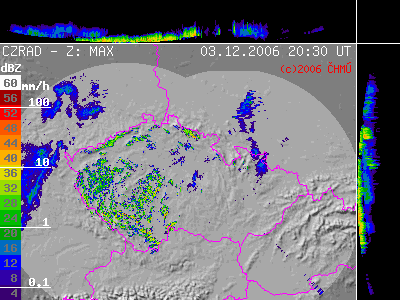
\includegraphics[width=0.6\textwidth]{./img/srazky/0612032030-gif.png}
    \caption[Ostře ohraničené buňky]{\centering Příklad ostře ohraničených buněk  \footnotemark}
    %\label{fig:Srazky}
\end{figure}
\footnotetext{\url{http://www.meteoradar.cz/obr/0612032030.gif}}

\item[Rušení radaru] jiným signálem na blízké frekvenci způsobují ostré radiální paprsky, případně spirály. Často tato rušení způsobují WiFi sítě.

\begin{figure}[h!]
    \centering
    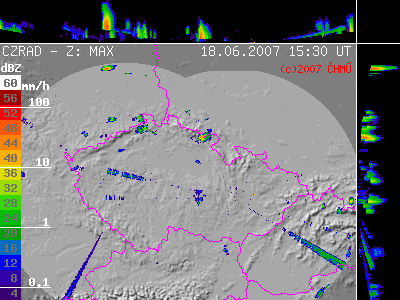
\includegraphics[width=0.6\textwidth]{./img/srazky/0706181530-gif.png}
    \caption[Rušení radaru]{\centering Příklad rušení radaru radiálními paprsky \footnotemark }
   %\label{fig:Srazky}
\end{figure}

\footnotetext{\url{http://www.meteoradar.cz/obr/0706181530.gif}}
\end{description}


\subsubsection{Dálkový průzkum země}
Je důležité zmínit možnost získávání informací o srážkách pomocí \acs{DPZ}. Tento obor z hlediska meteorologie zaujímá zcela jiný náhled na měření srážek oproti předchozím metodám. \acs{DPZ} v meteorologii umožňuje globální pohled na meteorologické jevy. Makro náhled na enviromentální jevy, např. cyklóny, tropické bouře, tornáda či pohyb mraků, je podstatný pro sledování a pochopení globálního vývoje klimatu. Do této kategorie spadá pozorování pomocí družic na oběžných drahách a leteckých prostředků pohybujících se v zemské atmosféře. Družice se dále dělí podle typu drah na polární a geostacionární, které jsou se pohybují nad stejným místem na zemi. Tyto satelity jsou umístěny nad rovníkem ve vzdálenostech okolo 36,000 km a pořizují snímky z dané hemisféry zeměkoule. Polární družice se pohybují na orbitách přes severní a jižní pól. Rotace Země těmto družicím umožňuje snímat jakékoliv místo na planetě Zemi. Výhoda těchto družic oproti geostacionárním spočívá v bližší oběžné dráze obvykle okolo 870 km nad povrchem a z toho plynoucí lepší rozlišení snímků. 
Meteorologické satelitní družice disponují různými druhy senzorů, které je dělí do kategorií podle měření různých meteorologických jevů např. teploty, srážek, mraků, radiace, sněhové pokrývky, atd. Měření se především liší  využitím různých kanálů, které pracují na rozdílných vlnových délkách elektromagnetického spektra.
 
\paragraph*{Princip} pozorování je založen na radiometrickém měření různých vlnových délek e krátkých časových intervalech pomocí zrcadel umístěných na družicích, které skenují daný region a odesílají digitální data zpět na Zemi.
\paragraph*{Elektromagnetické spektrum} se v meteorologii typicky využívá ve vlnových délkách spadajících do viditelného a infračerveného spektra. Satelitní snímky se v oblasti meteorologie dělí na snímky viditelného spektra, infračerveného spektra a z hlediska určování srážek nejpodstatnější snímky zprostředkované kanály absorbující primárně vodní páry.

\paragraph*{Satelitní snímky} v oblasti meteorologie se dělí na snímky viditelného spektra, infračerveného spektra a snímky pobízené kanály absorbující vodní páry. 
\begin{description}
\item[IR odhady srážek] Odrazivost infračerveného spektra je velmi vhodná pro odhad srážek z mraků, které jsou chladnější a vyskytují se ve vyšších výškách. Tento fakt je výhodný, jelikož vrcholky mraků korelují s vyšším výskytem srážek. Pro přesnější odhad srážek se prostorově v různých časových okamžicích průměrují \acs{IR} teploty [k], které se poté porovnávají s měřením srážek, čímž se docílí vyšší korelace se skutečnými srážkami.



\item[Mikrovlnné kanály] využívané pro odhad srážek se pohybují ve vlnových délkách v jednotkách [GHz]. Některé kanály jsou umístěny v oknech vlnových délek, kde atmosférické plyny absorbují velmi málo záření. Tato okna vlnových délek umožňují prohlédnutí přes mraky až na zemský povrch. Jejich doplňkem jsou naopak okna, jejichž vlnové délky silně absorbují srážky. Ta jsou výhodná k odhadu srážkových úhrnů. Odhad srážek pomocí mikrovln je nejpřesnější nad oceány, kde odrazivost pozadí srážek je rovnoměrná. Nad pevninami je odrazivost variabilní a tím se zhoršuje přesnost odhadu srážek. Rozlišení satelitních snímků pořízených na frekvencích mikrovln se typicky pohybuje okolo 5x6 [km].
\end{description}


\subsection{Mikrovlnné spoje}
Mikrovlnné (MV) spoje jsou rádiové systémy široce využívané v oblasti telekomunikací (zejména 
mobilními operátory) k bezdrátovému propojení dvou vzdálených stanovišť. MV spoje operují na 
frekvencích, kde dešťové kapky představují hlavní zdroj útlumu signálu. Analýza útlumu signálu 
umožňuje poměrně přesně odhadnout průměrnou srážkovou intenzitu podél spoje. Vzhledem 
k hustotě sítě MV spojů (např. v Praze řádově stovky až tisíce) jde o relevantní zdroj srážkové 
informace, který má velký potenciál zlepšit prostorovou informaci o srážkových intenzitách. Využití 
standardních GIS nástrojů může výrazně zefektivnit jak zpracování dat, tak jejich následnou správu. 
Vhodná vizualizace těchto dat je důležitým předpokladem pro vylepšení stávajících modelů pro 
převod útlumu signálu MV spojů na srážkové intenzity i pro další využití těchto dat.
 
\begin{figure}[h!]
    \centering
    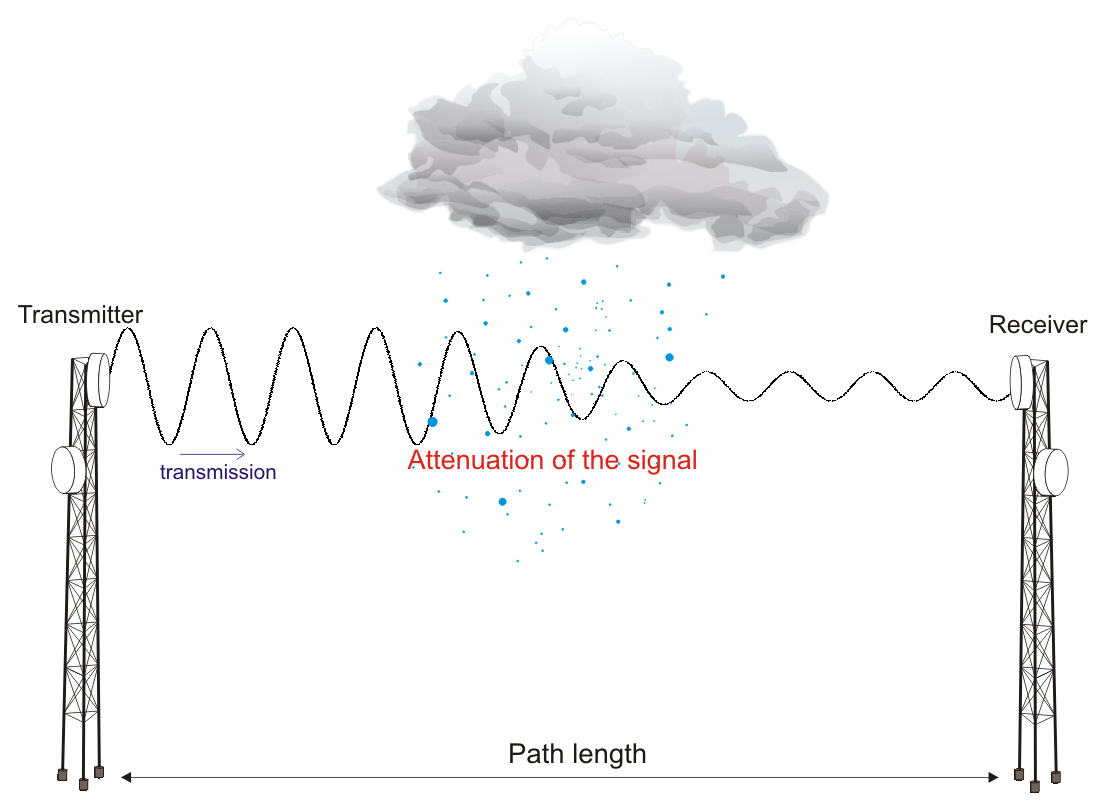
\includegraphics[width=0.7\textwidth]{./img/srazky/microwave_link.png}
    \caption[Rušení radaru]{\centering Absorbce elektromagnetického spektra atmosférickými plyny  \footnotemark }
 \end{figure}   
\footnotetext{\url{http://www.goes-r.gov/users/comet/tropical/textbook_2nd_edition/media/graphics/emspect.gif}}
    
\subsubsection{Princip}
Mikrovlny jsou elektromagnetické vlny o délce v rozpětí od 1 [mm] do 1 [m]. Tomu odpovídá frekvence 0.3  až 300 [GHz]. V oblasti telekomunikací především mobilních operátorů se tohoto typu vln využívá ke komunikaci mezi jednotlivými vysílači a vysílači s mobilními telefony. Pro rekonstrukci srážek se využívá prvního případu, tedy komunikaci mezi vysílači. Tyto mikrovlnné spoje pracují na frekvencích v rozsahu 24-39 [GHz] (Praha). Hlavním zdrojem útlumu tohoto frekvenčního rozsahu jsou dešťové kapky. Jednotlivé spoje se vždy skládají ze dvou vysílačů. Vysílač neustále odesílá MV vlny, které jsou nositelem informace zajímavé především pro telekomunikace. Vedlejším produktem této komunikace je údaj o intenzitě signálu, jehož základní jednotkou je decibel [dB]. Zaznamenat hodnotu intenzity signálu odeslaného a druhým přijímačem přijatého je možné bez dalších instalací hardware. Pomocí fyzikálně-parametrického modelu dle ITU-R\cite{itu} lze vypočítat průměrné srážky na pomyslné linii MV spoje.

\subsubsection{Výpočet srážek}
Vysílané hodnoty intenzit signálu \emph{tx} jednotlivých MV spojů jsou konstantní. Jednotlivé spoje jsou charakterizovány hodnotami:
\begin{itemize}
\item \textbf{Frekvence} \emph{f} rozsahu 24-39 [GHz]
\item \textbf{Polarizace} signálu ve vertikální \emph{V} či horizontální poloze \emph{H}
\item \textbf{Vzdálenost} \emph{L} která je vypočtená v daném souřadnicovém systému v kilometrech[km]
\end{itemize}
Přijaté hodnoty intenzit \emph{rx} jsou nositelem informace o útlumu signálu. Rozdílem vyslané \emph{tx} a přijaté \emph{tx} intenzity dostaneme výsledný útlum \emph{$A_{r}$} v jednotkách decibel[dB].
\begin{equation}
 A_{r}=tx-rx
\end{equation}
Dalším krokem je určení \emph{baseline}, tedy hodnoty \emph{ $A_{0}$ }  ,která představuje konstantní útlum intenzity signálu MV spoje bez vlivu útlumu signálu dešťovými kapkami. Tato konstanta je v jednotkách decibel[dB]. Parametrická konstanta  \emph{$A_{w}$ } je hodnota nadměrného útlumu způsobená mokrou anténou. Z toho plyne výsledný útlum \emph{$A_{m}$ }[dB].
\begin{equation}\label{eq:Ar}
 A_{m}=A_{r}-A_{0}-A_{w}
\end{equation}
 Výsledný útlum je třeba převést na specifický útlum \emph{$\gamma_{R} $} [dB/km] pro danou vzdálenost \emph{L} mezi vysílači MV spojů. 
\begin{equation}
\gamma_{R} =\frac{A_{m}}{L}
\end{equation}
Dle doporučení ITU P.838 \cite{itu} je specifický útlum  \emph{$\gamma_{R} $} a intenzitu srážek  \emph{R} [$mm \cdot h^{-1}$] ve vztahu
\begin{equation}\label{eq:gamma}
\gamma_{R}=kR^{\alpha}
\end{equation}
Koeficienty \emph{k} a \emph{$\alpha$} jsou určeny jakožto funkce frekvencí \emph{f}[GHz] v rozsahu od 1 do 1000[GHz], z následujících rovnic.

\begin{equation}
log_{10}k=\sum_{j=1}^{4} a_{j} exp\left [ -\left ( \frac{log_{10}f-b_{j}}{c_{j}} \right )^{2} \right ]+m {_{k}}log_{10}f+c_{k}
\end{equation}

\begin{equation}
\alpha=\sum_{j=1}^{5} a_{j} exp\left [ -\left ( \frac{log_{10}f-b_{j}}{c_{j}} \right )^{2} \right ]+m{_{\alpha }}log_{10}f+c_{\alpha }
\end{equation}
kde:

\emph{f}: frekvence [GHz]

\emph{$\alpha$}:  dle polarizace \emph{$\alpha_{H}$} nebo \emph{$\alpha_{V}$}

\emph{k}: dle polarizace  \emph{$k_{H}$} nebo \emph{$k_{V}$}

{\raggedright{}Hodnoty pro dané konstanty jsou součástí dokumentu ITU-R \cite{itu}.}
\bigskip

{\raggedright{}Inverzním vztahem rovnice \eqref{eq:gamma} dostaneme výslednou intenzitu srážek \emph{R} [$mm \cdot h^{-1}$]. }


\begin{equation}
R=\left ( \frac{\gamma_{r}}{k} \right )^{\frac{1}{\alpha }}
\end{equation}


\subsubsection{Chyby}
\label{subsec:chyby}
Metoda odhadu srážek je založena na předpokladu, že dešťové kapky tlumí signál. Dešťové kapky nabývají mnoha variací velikosti a tvarů. Signál může být tlumen škálou objektů od vodní páry, jejímž zdrojem je povrch Země, přes mrholení až po velké dešťové kapky. Vztah mezi intenzitou srážek \emph{R} a útlumem \emph{$\gamma_{R} $} je funkcí frekvence, polarizace a rozložení dešťových kapek\acs{DSD} s parametry \emph{a} a \emph{b}. Pro tento vztah na frekvencích mezi 25 a 40 GHz platí takřka lineární závislost. V tomto frekvenčním rozmezí je model téměř nezávislý na teplotě, rozložení dešťových kapek a empiricky vykazuje chybovost méně než 10\emph{\%}. Na nízkých frekvencích okolo 10 GHz přesahuje chybovost 20\emph{\%}. Přesnost určování srážek výše zmíněným modelem dle ITU P.838 je při těchto nízkých frekvencích mnohem více náchylná na rozložení kapek\acs{DSD}.\cite{dsd} 


\paragraph*{Nejistoty modelu} založeného na vztahu \eqref{eq:Ar} jsou především v závislosti \emph{$\gamma_{A_{m}} $},\emph{$A_{w} $} na rozložení kapek \acs{DSD} podél MV spoje.

\paragraph*{DSD} způsobují nejistoty při určení výsledného útlumu signálu \emph{$\gamma_{A_{m}} $}. Tyto chyby jsou zapříčiněny integrací jednotlivých úseků tlumících signál na linii MV spoje. \cite{mv1}

\paragraph*{Mokré antény}jsou značným zdrojem nejistot. Na vysílačích nejsou antény nijak kryty a při dešti moknou. Na anténách se vytváří tenký film vody, který ovlivňuje výsledný útlum signálu. Vytvoření modelu pro eliminaci tohoto problému se do značné míry podařilo (Schleiss et al., 2013)\cite{wetat}. Součástí výzkumu, pod který tato práce částečně spadá, bude instalace krytu na antény, který by mohl zamezit jejich moknutí. Tato možnost doposud nebyla součástí žádné vědecké práce.

\paragraph*{Určení baseline } \emph{ $A_{0}$ } je jedním z důležitých a nejvíce ovlivňujících činitelů při výpočtu výsledné srážky \emph{R}. Tato hodnota se zcela mění v čase a je závislá na koncentraci vodní páry v atmosféře a scintilaci. Útlum vysílaných a přijímaných vln ovlivňuje také teplota prostředí jímž vlna prochází. Dalším činitelem, který může způsobovat kolísání signálu, je vítr.
Pro určování baseline se využívá různých metod, například \acs{HMM} \cite{comparsinmv}, Retrieval Alghorithms \cite{countryw}. Metody Určení baseline se dají klasifikovat na automatizované a uživatelské. Automatizovaným určováním baseline se myslí především algoritmy, které jsou schopny detekovat, mokré a suché období. Některé tyto algoritmy využívají statistických prostředků a jiné například určují období dešťů pomocí dat ze srážkoměrů \cite{countryw} či radaru. 


\subsection{Srovnání}
Tato podkapitola je zaměřena na shrnutí vlastností jednotlivých metod a jejich porovnání s metodou MV spojů. Hodnocení jednotlivých metod je založeno na kritériích, která jsou pro měření srážek typická.
\begin{itemize}
\item\textbf{Časová spojitost}
\item\textbf{Interval sběru dat}  
\item\textbf{Prostorové rozlišení}
\item\textbf{Disponibilita jednotlivých metod}
\item\textbf{Chyby}
\end{itemize}
V současné době jsou v oblasti hydrometeorologie požadována velmi přesná data ve vysokém prostorovém a časovém rozlišení. Tyto nároky jsou především vytvořeny požadavky hydrologických modelů, jejichž výsledky napomáhají k lepšímu operativnímu řízení odtoku v urbanizovaných územích. Kvalita vstupů dat do těchto modelů je rozhodující pro jejich přesné výsledky, které jsou základem přijímaných opatření vedoucích ke snížením povodňových škod. .

\paragraph*{Srážkoměrné sítě} 
tyto požadavky splňují jen částečně. Moderní srážkoměry splňují kritérium schopnosti pokrytí spojité časové řady až v minutových intervalech. Hlavním záporem těchto sítí je nedostatečné pokrytí. Jelikož datovým výstupem těchto sítí jsou bodová data, je zde problém v nedostatečné hustotě pokrytí srážkoměry, která prakticky nemůže být nikdy odstraněna. Prostorová variabilita srážek, kde se jednotlivé mohou řádově lišit už ve stovkách metrů, má za následek zachycení či naopak nezaznamenání lokálních maxim, které jsou ve výsledné plošné rekonstrukci zdrojem nezanedbatelných chyb. Měření moderními srážkoměry může být při správné volbě umístění velmi přesné. Toho se v současnosti využívá jako referenčního indikátoru srážek pro kalibraci radarů, nebo k určování baseline při odhadu srážek MV spoji (\ref{subsec:chyby},Baseline).

\paragraph*{Radary}
jsou současnou nejvíce využívanou metodou pro plošné vyjádření srážek. Snímky se pořizují v 5-15 minutových krocích a tento časový interval nelze z fyzikální podstaty radaru zmenšit. To poukazuje na možnou chybovost, jelikož srážky během 5 minut mohou nabývat jiných hodnot až o řád. Mezi kladné vlastnosti radaru bezesporu patří mimo klasické rozlišení v horizontálním směru (plošné) také i měření odrazivosti vertikálních profilů. Tuto vlastnost v rozlišení 1 km pro vertikální a 2 km pro horizontální ostatní metody neumožňují. Prostorové rozlišení je dále možno pozorovat jen pomocí některých meteorologických družic, které skenují Zemi pod sklonem jiným než nadir. Jejich rozlišení je ale v jednotkách horší. Pro zpřesnění radarových srážek pro potřeby hydrologie je navíc potřeba jejich adjustace na pozemní srážkoměry. Obecně vzato je výsledné plošné rozlišení radaru pro městské odtokové modely nedostačující.   

\paragraph*{Družice} se z výše zmíněnými metodami nedají zcela korektně porovnávat. Družice na oběžných drahách slouží především k náhledu na chování klimatu. Snímky těchto družic jsou nositelem informací v rozlišení, reflektující spíše obecnou informativní podstatu, např. pohybu front, vývoje cyklónu a k náhledu na globálnímu přehledu o vývoji počasí, či dlouhodobě klimatu.
Jednou z výhodou rekonstrukce srážek pomocí metody \acs{IR} pásem je poměrně vysoká frekvence záznamu snímků v intervalu 15 minut na jakémkoliv místě na Zemi. Při porovnání s pozemním meteo radarem je slabost této metody ve špatném, u některých družic nulovém, detekování vertikálních profilů srážkových mraků, což vede k podceňování výsledných srážkových úhrnů.


\subsubsection{Mikrovlnné spoje}
Metoda odhadu srážek pomocí MV spojů byla předmětem výzkumu už v 80. letech 20. století. Prakticky byla použita až při využití komerčních telekomunikačních spojů v posledním desetiletí. Budoucnost této metody je především v pokrytí v osídlených oblastech, kde je právě přesnost odhadu srážek nejvíce vyžadována. Pokrytí s vývojem mobilních technologií se stále zlepšuje. Data jsou sbírána ve velmi malých intervalech běžně po 10[s]. Při využití rozsáhlých sítí až stovky spojů ,např v Praze, umožňuje tato metoda relevantní plošnou časoprostorovou informaci o srážce.
 
\paragraph*{Potenciál MV v hydrometeorologii} zasahuje do všech oblastí vědních oborů, kde se využívají srážky jakožto vstupní časové řady. Tato metoda je v současné době spíše vhodná pro lokální využití nežli regionální. Vyplývá to z absence pokrytí sítí mimo osídlené oblasti. 

Jedním z velkých potenciálů této metody je zlepšení přesnosti prostorové informace o srážkách ve vysokém rozlišení. To žádné současné metody odhadu srážek neumožňují. Výsledky stude\cite{mv2} poukazují na možnosti částečného nahrazení současných metod nebo možnosti vzájemného se doplňování jednotlivých metod, což by vedlo zlepšení přesnosti odhadu srážek. 

Jelikož tyto MV spoje operují těsně nad zemským povrchem, vypočtené intenzity by mohly být pomocí nástrojů \acs{GIS} přiřazovány do jednotlivých subpovodí. To by zpřesnilo vstupy do srážko odtokového modelu a umožnilo lépe modelovat členitá povodí na místě velkých aglomerací.

Možnosti využití MV spojů v oblasti meteorologie nekončí u odhadu srážek. Pomocí MV lze také detekovat pevné částice, sníh, či vodní páry. Tyto možnosti by mohly napomoci k lepšímu pochopení jevů spojených s přívalovými srážkami.\cite{mv2}
\begin{figure}[h!]
    \centering
    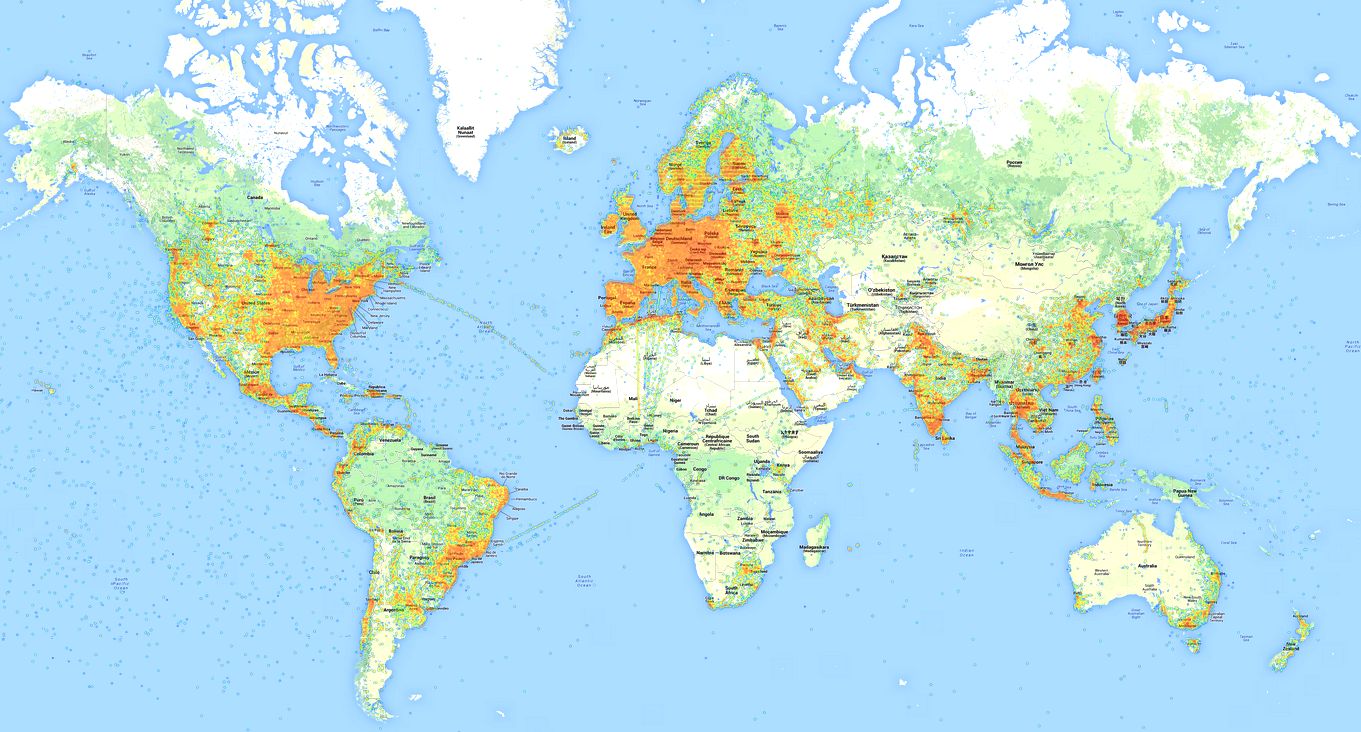
\includegraphics[width=1\textwidth]{./img/srazky/opensignalmap.png}
    \caption[Porytí tel. sítí]{\centering Mapa celosvětového pokrytí signálu telekomunikačních mobilních operátorů. Pokrytí je vyjádřeno oranžovou a žlutou barvou. \footnotemark }
 \end{figure}   
\footnotetext{Obrázek byl sejmut z webové aplikace OpenSignal. \url{http://opensignal.com/}}

Velkým potenciálem je takřka nulová finanční náročnost pro sběr dat. Telekomunikační sítě mobilních operátorů jsou v hustěji osídlených částech světa běžné. V rychle se rozvíjejících zemích třetího světa se v průběhu času stanou telekomunikační sítě samozřejmostí a využití metody odhadu srážek by se mohlo stát více dostupnou oproti budování radarů, pozemních stanic, či sítě srážkoměrů.
 


\setcounter{footnote}{1}







\newpage
\section{Použité technologie}
Tato kapitola je úvodem k praktické části práce a je zaměřena na nástroje využité k implementaci Python modulu do GRASS GIS. Jsou zde popsány základní principy a charakteristiky jednotlivých nástrojů, kde je kladen především důraz na návaznost k praktické části práce.

\subsection{Systém GRASS GIS}
\textbf{GRASS} (Geographic Resources Analysis Support System) GIS \footnotetext{\url{http://grass.osgeo.org/}} je multiplatformní geografický systém, šiřitelný pod všeobecně veřejnou licencí \acs{GNU GPL}. Systém je primárně určený pro správu 2D/3D rastrových a vektorových geodat, jejich zpracování, analýzu a vizualizaci. K těmto účelům knihovna GRASS GIS disponuje několika stovkami modulů, které jsou současní stabilních verzí. Mimo to je volně dostupných mnoho jiných modulů, které jsou vyvíjeny uživateli v rámci GRASS \textit{AddOns} a mohou se stát součástí stabilních vývojových verzí GRASS. 

GRASS GIS je na poli GIS software zcela unikátní a to především díky svému rozsahu, čemuž vděčí především dobrovolným vývojářům z komunity GRASS po celém světě, kteří tento dlouholetý projekt vyvíjí. Za jeho kvalitu jsou důkazem uživatelé mezinárodního charakteru jako \textit{NOAA}\footnote{\url{http://www.noaa.gov/}} či \textit{NASA}\footnote{\url{http://www.nasa.gov/}}. 

\begin{figure}[h!]
    \centering
    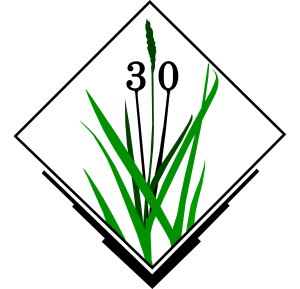
\includegraphics[width=0.3\textwidth]{./img/grass/grasslogo.png}
    \caption[Logo GRASS]{\centering Logo GRASS GIS vydané symbolicky k 30. výročí od založení projektu. \footnotemark }
 \end{figure}   
\footnotetext{\url{http://grass.osgeo.org/uploads/images/30-years-grass-gis-logo-black-300px.png}}


\subsubsection*{Historie}
Vývojová linie GRASS GIS je stálá od poloviny osmdesátých let minulého století, kde byl vyvinut primárně pro americkou armádu, která jej využívala pro územní správu a plánování. Během 90. let se postupně na vývoji projektu podíleli americké federální agentury, univerzity a soukromé společnosti. Hlavní vývoj projektu byl řízen z výzkumných laboratoří (USA-CERL\footnotetext{\url{http://www.cecer.army.mil/}}) Champaign, Illinois.\cite{grasshist}.
Mezníkem historie GRASSu byl rok 1995, ve kterém se laboratoře CERL zřekli tohoto projektu, čehož  následek byl přesun vývoje na akademickou půdu. Rok před začátkem nového tisíciletí byla vydána první verze pod licencí GNU GPL, pod kterou je vyvíjen dodnes. V letech 2008 se GRASS GIS zařadil do nadace \acs{OSGeo}, pod kterou spadá mnoho významných volně šiřitelných geografických projektů.\footnotetext{\url{http://www.osgeo.org/}}. Letošním rokem oslavil GRASS dlouhých 30 let vývoje, které zaštítil vydáním verze \textit{GRASS GIS 7.0.0 beta1}.\footnotetext{url{http://grass.osgeo.org/news/32/56/GRASS-GIS-7-0-0-beta1/}}

\subsubsection*{Základní terminologické pojmy}
Hlavním cílem této sekce je představit čtenáři základní filosofii uživatelského rozhraní systému GRASS GIS.
\paragraph*{Data} ke kterým GRASS přistupuje, jsou definována  pevně stanovenou  adresářovou  strukturou. Pro práci v tomto systému, je prvně zapotřebí definovat trojici nastavení. V grafickém rozhraní GRASS \acs{wxGUI} je implementován průvodce nastaveni pro jednotlivými kroky 

\begin{enumerate}
\item \textbf{Database} v prostředí GRASS je stanovena proměnou \texttt{\$GISBASE}. Jedná se o standardní adresář umístěny na disku, který je pojmenován (\textit{grassdata}). V tomto adresáři jsou uloženy veškerá uživatelská data mimo externě připojené databáze (\textit{např. PostgreSQL, MySQL }).

\item \textbf{Lokace} je adresář umístěný v souborové databance. Lokace je definována proměnou   \texttt{\$LOCATION\_NAME}
a obsahuje data, která nesou informace o souřadnicovém systému a velikosti zájmového území. Pro nastavení lokace je v grafickém rozhraní průvodce nastavením lokace (\textit{Location wizard}), kde je možné zvolit souřadnicový systém pomocí možností.
\begin{itemize}
\item seznam jednotlivých obecně známých projekcí 
\item zadáním unikátního kódu z databáze \acs{EPSG}. \footnote{\url{http://www.epsg-registry.org/}}
\item načtením externích georeferencovaných dat
\item definováním parametrů projekce s využitím pravidel PROJ.4\footnote{\url{http://trac.osgeo.org/proj/}}
\item pomocí \ac{WKT} souboru .prj, který je součástí shapefile jako doplňkový.
\end{itemize}

\item \textbf{Mapset} definovaný proměnou \texttt{\$MAPSET} představují jakýsi profil uživatele, či profil ucelených analýz  v dané lokaci. Každá lokace musí obsahovat mapset, který má unikátní název \texttt{PERMANENT}. Do tohoto mapsetu se z pravidla ukládají vstupní data, ke kterým se z ostatních pracovních mapsetů přistupuje.
\end{enumerate}



\paragraph*{Modul} je nedílnou součástí software architektury tohoto geoinformačního systému. Volba implementace pomocí jednotlivých modulů pochází z doby, kdy vypočtení technika byla v počátcích a šetrné využití operační paměti a procesorového výkonu bylo nezbytností. Jádro systému je napsáno procedurálně v jazyce C k němuž jsou  jednotlivé funkcionality integrovány pomoci \acs{API}, které je v jazyce C a Python. Funkcionality-moduly jsou logicky rozděleny do kategorií, podle účelu jejich využití.

\begin{table}[h]
\centering
\begin{tabular}{|cccccccc|}
\hline
db. & d. & g. & i. & ps. & r3. & r. & v. \\
\hline \hline
database & display & general & imagery & postscript & 3D raster & raster & vector \\ \hline
\end{tabular}
\caption{Přehled jednotlivých skupin modulů a jejich prefixů v GRASS GIS}
\label{tab:module}
\end{table}


Nyní také nově v \textit{GRASS 7} moduly \textit{Temporal GRASS} s prefixem \texttt{*t}. Jednotlivé moduly se spouštějí pomocí příkazové řádky a nebo v grafickém rozhraní \textit{wxGUI} . Rozhraní modulů umožňuje uživatelský vstup pomocí přepínačů a parametrů např. \texttt{mv.precip -p database=letnany}. Parametry se dělí na povinné (\texttt{required}) a volitelné (\texttt{optional}). V modulech jsou také globální přepínače, které jsou pro všechny moduly definovány jednotně. Mezi nejčastěji využívané patří \texttt{--help}, který do terminálu vypíše veškeré informace o vstupních parametrech včetně jejich  popisu.


\subsection{GRASS Python API}
\subsection{PostgreSQL}
PostgreSQL\footnote{\url{http://www.postgresql.org/}} je open-source projekt, který vznikl v roce 1986. Tento projekt je dnes celosvětově uznávaný, čehož důkazem je využití systému ve světových projektech jako \textit{SourceForge}\footnote{\url{http://sourceforge.net/}}, \textit{Debian}\footnote{\url{http://www.debian.org/}} či \textit{Open Street Map}\footnote{\url{http://www.openstreetmap.org\#map=15/49.9503/14.5322}}. Kvalita systému a rozsáhlá dokumentace je především dílem komunity dobrovolníků, díky kterým je PostgreSQL schopno konkurovat i proprietárním databázovým systémům. Tomu také mimo jiné přispívá fakt, že se řadí mezi multiplatformní systémy.\cite{postgre}

\begin{figure}[h!]
    \centering
    
\includegraphics[width=0.2\textwidth]{./img/implementace/postgresql.png}
    \caption[Logo PostgreSQL]{\centering Logo PostgreSQL }
 \end{figure}   


\subsubsection{Princip databáze PostgreSQL}
\paragraph*{Architektura}
PostgreSQL je \ac{ORDBMS} tedy systém relační databáze doplněný o objektově orientovaný model. Funguje na principu klient-server, kde každý klient je obsluhován samostatným procesem, který se stará o zpracování dotazu. Tedy \textit{host} server se skládá ze dvou částí: \textit{postmaster} a \textit{postgres}.  Když klient odešle požadavek k přístupu k databazi na server, \textit{postmaster} na serveru založí nový procese, \textit{postgres} a ten přímo komunikuje s klientem. Z toho plyne že proces \textit{postmaster} musí nepřetržitě běžet, oproti tomu  proces \textit{postgres} začne a skončí na příkaz klienta. 


\paragraph*{Zpracování dotazu}
Dotazy se dělí na dělí podle jejích typu na optimalizované a neoptimalizované. Do skupiny optimalizovaných spadají příkazy z \ac{DML}. Ty jsou charakteristický právě s pohybem/manipulací s daty. Patří mezi ně \texttt{SELECT}, \texttt{INSERT}, \texttt{UPDATE}, \texttt{DELETE} a další méně využívané. \ac{DDL}  představuje skupinu neoptimalizovaných dotazů, což plyne z jejich funkčnosti. Patří mezi ně především \texttt{CREATE}, \texttt{ALTER}, \texttt{DROP} a další. \cite{bares}


\begin{table}[h]
   \centering
\begin{tabular}{|ccll|}
\hline
definice & optm* & příkaz & popis \\ \hline \hline
\multirow{4}{*}{DML} & \multirow{4}{*}{$+$} & SELECT & vybírá data z databáze \\
 &  & INSERT & vkládá do databáze nová data. \\
 &  & UPDATE & editace data v databáz \\
 &  & DELETE & odstraňuje data \\ \hline
\multirow{4}{*}{DDL} & \multirow{4}{*}{$-$} & CREATE & vytváření nových objektů \\
 &  & ALETER & změny existujících objektů \\
 &  & DROP & odstraňování objektů \\
 &  & TRUNCATE & mazání všech záznamů z tabulky \\ \hline
\end{tabular}

\caption{Zařazení a popis SQL příkazu do kategorii.
*( ne/optimalizovaných )}
\label{tab:prikazy}
\end{table}


\begin{description}
\item[Parser]zastupuje funkci validátoru syntaxe. Zkontroluje správnou syntaxi vstupu a pokud je platná, transformuje příkaz na stromovou strukturu (\textit{query tree}). Součástí kontroly syntaxe spočívá i testováním existence jednotlivých výrazů, tabulek, schémat, atributů a dalších.

\item[Traffic Cop] identifikuje dotaz do výše zmíněných kategorií, tedy optimalizované\-/neoptimalizované.

\item[Utility Commands] je proces, který zpracovává jednoduché dotazy ze skupiny neoptimalizovaných. Z podstaty věci tyto příkazy nelze  optimalizovat.

\item[Planner/rewriter] také optimalizátor má za úkol vygenerovat optimální exekuční řešení. Pro vyhledání optimální cesty se využívá síťových analýz, kde jednotlivé cesty jsou  ohodnoceny a algoritmus vybere obecně tu nevýhodnější.

\item[Exekutor] pracuje pouze s \acs{DML}. Obdrží od výše zmíněného \textit{planneru} plán nejvýhodnější cesty a začne daný strom procesů zpracovávat od horního uzle. Mechanismus je  nastaven tak, že při procházení stromu pro každý uzel je exekutor spouštěn jednou a vrací se mu jeden záznam/řádek. V praxi tak exekutor prochází větve podle definovaných podmínek střídavě(dle podmínek). Tedy k jednomu řádku hledá odpovídající podle podmínky. 
\end{description}


  
\begin{figure}[h!]
    \centering
    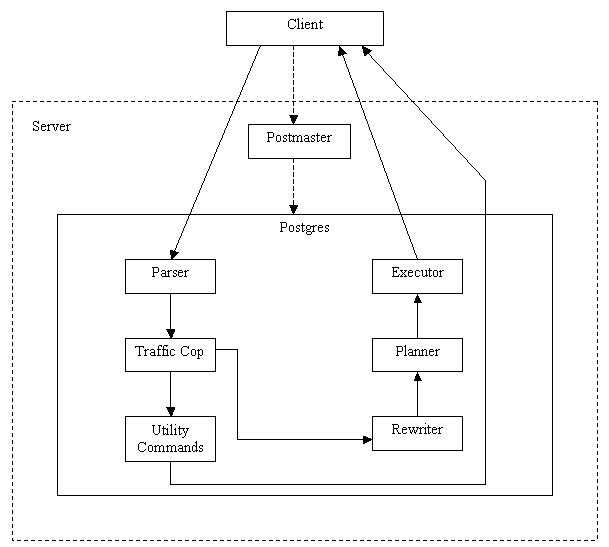
\includegraphics[width=0.6\textwidth]{./img/implementace/postgremodel1.jpg}
    \caption[Dotaz PostgreSQL]{\centering  Zpracování dotazu \footnotemark}
 \end{figure}   
\footnotetext{\url{http://reshmaparveen.blogspot.cz/2009/12/normal-0-false-false-false.html}}




\subsubsection{Vlastnosti}
PostgreSQL je \ac{ORDBMS} je systém relační databáze doplněný o objektově orientovaný model. Ten je specifikován v rozšíření standardu SQL3 z roku 1999\cite{sql1999}. Objektový model podporuje objekty, třídy a dědičnost v databázových schématech. Objektově-relační systém pro zprávu databáze  poskytuje střední cestu mezi relační a plně objektově orientovanou databází. To je vhodné v možnosti vytváření vlastních datových typů a metod, které umožňují vyšší míry abstrakce. Nechybí podpora implementace vlastních procedur bud s využitím vlastního jazyka PL/pgSQL nebo využít externí podpory C/C$++$ (knihovny libpq a libpq$++$), Python (PyGreSQL), Perl (pgsql\_perl5).


\paragraph{Objekty} umožňují vytvoření nových datových typů. Konverze, přetypováním, indexy, funkce, agregační funkce, operátory a další.  
\paragraph*{Funkce} umožňují spouštění bloků kódu, které mohou být jak v nativním jazyce PL/pgSQL, tak i v ostatních výše zmíněných podporách. Funkce po spuštění vracejí výsledek v řádcích, tedy tabulkou, kterou je možné využít k dalším příkazům. Možnost je vytvoření vlastních funkcí, či využití funkci z nativní knihovny PostgreSQL nebo také funkce externě funkce z přidaných extenzí (\texttt{EXTENSION}).
\paragraph*{Indexy} PostgreSQL umožňuje vytvářet pomocí algoritmu \textit{B-tree}, \textit{hash}, \textit{GiSTm} a \textit{GIN} \footnote{\url{http://www.postgresql.org/docs/9.1/static/sql-createindex.html}}, nebo lze vytvářet i vlastní. Princip indexu spočívá ve vytvoření specifického sloupce v tabulce, jehož jediný úkol je optimalizovat prohledávání daného sloupce. 
\paragraph*{Pravidla} umožňují nad jednotlivými tabulkami nebo pomocí \texttt{SELECT} vytvářet náhledy (\texttt{VIEW}). Principiálně jde o virtuální tabulky, které jsou logicky odkazují na vyprané sloupce v jiných tabulkách. V \textit{PostgreSQL 9.3 } jsou nově implementované materializované pohledy (\texttt{MATERIALIZED VIEW}), které představují část jak charakteristiky tabulky a tak pohledu pohledu. Data materializovaných pohledů jsou fyzicky uloženy na disku. Jejich hlavní výhoda spočívá v možnosti obnovení (\texttt{REFRESH}), čímž doje k obnovení tabulky na základě logických vazeb z vytvoření.
\paragraph*{Triggery} nebyli spouštěče mají funkcionalitu v podobě kontroly událostí, na které reagují podle své definice. Například při vytvoření nového záznamu provedou definovanou operaci v databázi. 
\paragraph*{Datové typy} definují druh nebo význam hodnot. V PostgreSQL je široká škála datových formátu. Specifickými pro tuto práci jsou: numerické, časové, logické, řadící(enumerate) a geometrické typy.

\subsection{Extenze PostGIS}
PostGIS\footnote{\url{http://postgis.net/}} je open-source rozšířením \texttt{EXTENSION} databáze PostgeSQL o podporu geografických objektů. Jde tedy o velice vhodný   nástroj pro využití v GIS. PostGIS implementuje specifikaci \textit{Simple Features for SQL}\footnote{\url{http://www.opengeospatial.org/standards/sfs} } konsorcia \acs{OGC}, která v současné době plní funkci standardizační organizace pro geoprostorová data. PostGIS 2D/3D je vektorovou databázovou nadstavbou, vedle které je i extenze PostGIS Raster. 

  
\begin{figure}[h!]
    \centering
    
\includegraphics[width=0.2\textwidth]{./img/implementace/postgis.png}
    \caption[Logo PostGIS]{\centering  Logo PostGIS \footnotemark}
 \end{figure}   
\footnotetext{\url{http://postgis.net/docs/manual-2.1/}}

\paragraph*{Geometrický model} 
Prostorový model je založen na specifikaci \acs{OGC} \textit{Simple Feature}, z toho plyne že model nepodporuje geometrickou topologii. OGC definuje jednotlivé operace mezi standardem SQL a prostorovými daty. Souřadnice jednotlivých objektů jsou ukládány v tabulkách, kde každá tabulka je specifická jedním typem geometrie(bod, linie, polygon atd.) a referenčním prostorovým systémem. Souřadnice jsou ukládány ve standardu \acs{WKT}. Spolu s  metadaty o geometrickém prvku jsou ukládány ve sloupci \texttt{geometry}, který je  nositelem informací o geometrickém typu a referenčním systému.\cite{postgis}

\begin{figure}[h!]
    \centering
    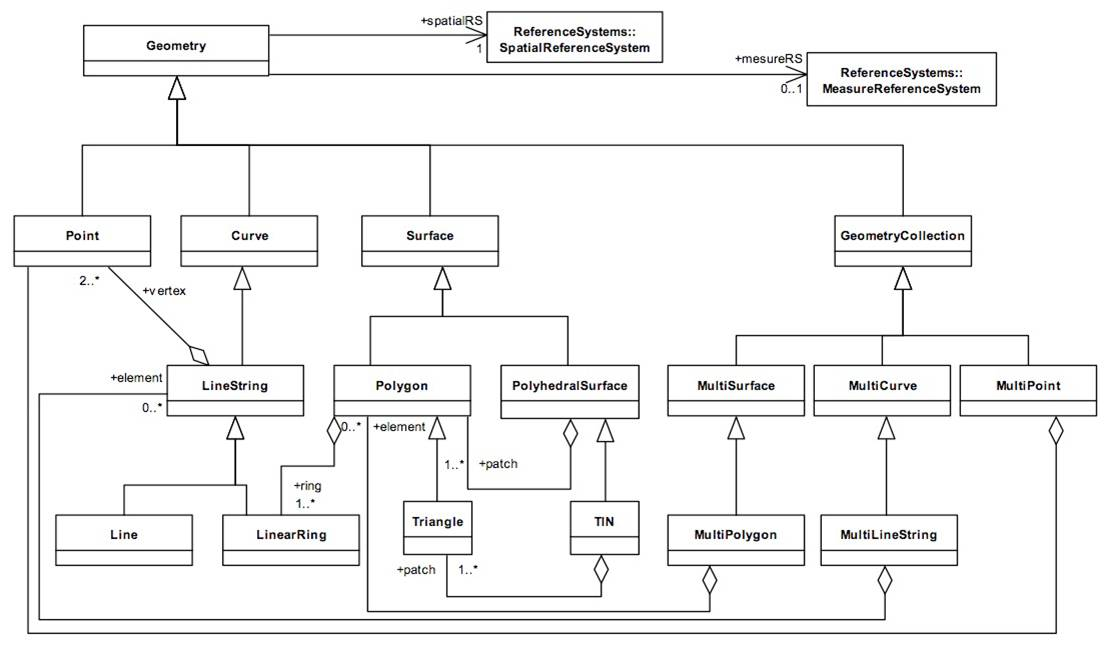
\includegraphics[width=0.8\textwidth]{./img/implementace/ogc1.jpg}
    \caption[Model PostGIS]{\centering Jednotlivé základní geometrické objekty jsou agregovány do složitějších tzv. Multi Obejct.     \footnotemark}
 \end{figure}   
\footnotetext{\url{http://www.opengeospatial.org/standards/sfs}}

\paragraph*{Souřadnicový systém} \texttt{SPATIAL\_REF\_SYS} je v PostGIS  definován v samostatných tabulkách. Obecně známé referenční systémy jsou již předdefinované, ostatní se dají dodatečně definovat a upravovat.

\begin{verbatim}
CREATE TABLE spatial_ref_sys (
  srid       INTEGER NOT NULL PRIMARY KEY,
  auth_name  VARCHAR(256),
  auth_srid  INTEGER,
  srtext     VARCHAR(2048),
  proj4text  VARCHAR(2048)
)
\end{verbatim}

Souřadnicové systémy a projekce jsou charakterizovány unikátním kódem \texttt{\acs{SRID}}, který je všeobecným standardem v GIS. Pro konverze mezi jednotlivými systémy slouží funkce \texttt{ST\_Transform}.\footnote{\url{http://postgis.org/docs/ST_Transform.html}}


\paragraph*{Geometrie} \texttt{geometry} je datovým typem, který představuje geometrickou složku objektu.  Charakteristika tohoto datového typu je dána standardem \textit{Simple Features} ve formátu \acs{WKT}.
Sloupec s geometrií je definován pomocí parametrů, které nastavují obecné a geometrické  specifika: název, \textbf{typ}, souřadnicový systém a další.
Pro definování \textbf{typu} objektu jsou k vytvořeny funkce \texttt{ST\_Make* }, kde \texttt{*} jsou níže uvedené typy standardu \textit{Simple Fetures}. 


\begin{verbatim}
POINT(0 0)                                               
LINESTRING(0 0,1 1,1 2)                                       
POLYGON((0 0,4 0,4 4,0 4,0 0),(1 1, 2 1, 2 2, 1 2,1 1))          
MULTIPOINT(0 0,1 2)                                              
MULTILINESTRING((0 0,1 1,1 2),(2 3,3 2,5 4))                       
MULTIPOLYGON(((0 0,4 0,4 4),(1 1,2 1,2 2)), ((-1 -1,-1 -2,-2 -2,))) 
GEOMETRYCOLLECTIONM(POINTM(2 3),LINESTRINGM(2 3,3 4))                
\end{verbatim}

\paragraph*{Funkce} v této jsou nadstavbě zaměřeny na operace s geometrii. Veškeré funkce mají prefix \texttt{ST\_} (\textit{spatial type}). Část z nich je funkcionalitou analogicky odvozena z nástrojů GIS. Funkce jsou podle svého účelu roztříděny do kategorii. Níže jsou demonstrovány nejzákladnější kategorie a funkce.
\begin{description}
\item[Měřičské] funkce jsou typické prostorovými výpočty; plocha \texttt{ST\_Area}, vzdálenost \texttt{ST\_distance}, vzdálenost na elipsoidu \texttt{ST\_length\_spheroid} a další. 
\item[Geometrické konstruktory] slouží k vytváření geometrie podle \textit{Simple Featura}; vytvoření bodu \texttt{ST\_MakePoint}, linie \texttt{ST\_MakeLine}, polygonu \texttt{ST\_MakePolygon} a dalších.
\item[Analytické] funkce jsou v PostGIS implementovány dle standartu SQL-MM  vyplývající z ISO99, standard o multimédiích. \cite{sqlmm}. V této kategorii jsou funkce typické prostředí GIS. Mezi ně například patří: buffer \texttt{ST\_Buffer}, validita geometrie \texttt{ST\_IsValid}, sjednocení \texttt{ST\_Union}.
\item[Konverze] umožňují transformace mezi referenčními system. Dále pak umožňují oboustrannou konverzi mezi binárními a textovými formáty. Například do \acs{WKT} 

\begin{verbatim}
SELECT  ST_AsEWKT (geom) FROM link
.......
.......
"SRID=4326;LINESTRING(14.4533605575562 50.0689735412598,
                      14.4754581451416 50.0387687683105)"
\end{verbatim}

\item[Agregační] funkce PostGIS jsou principiálně stejné jako standardní SQL(průměr, max, min) s rozdílem, že jsou zaměřeny na geometrická data. Příkladem je funkce pro sjednocení \texttt{ST\_Union}.
\end{description}












\newpage

\setcounter{footnote}{1}
\section{Plošné interpolace }
Plošné interpolace slouží k odhadu hodnot v prostoru, jež jsou pomyslně ohraničeny výchozími daty, které se uvažují jako referenční. Nutnost odhadovat hodnoty má logickou návaznost na problematiku sběru dat.  Podobně tomu je i v oblasti hydrometeorologie\ref{subsec:11}. Charakteristickým rysem interpolací v GIS systémech je datový vstup reprezentovaný bodovým polem (vektor) a výstup v podobě rastru (grid). Interpolace se také využívají k převzorkování rastrů do jiného rozlišení.

Dalším pojmem který si je interpolaci blízky, je extrapolace. Extrapolací je myšlen postup, kdy jsou odhadovány data mimo prostorovou doménu referenčních bodů. Extrapolace oproti interpolaci je  typicky méně přesná.

Pochopení teoretický  principů, na  kterých jsou interpolace založené, je  nezbytným krokem  k dosažení kvalitních výsledků v analytické části. Důležité je především znát charakteristiky, ze kterých vyplývají meze jednotlivých metod. Tato kapitola je specifická teoretickým pohledem do problematiky plošných interpolací, s primárním zaměřením na ty, kterými disponuje systém GRASS GIS pro vektorová bodová data. 



\subsection{Metody}
Jednotlivé interpolační metody se obecně mohou kategorizovat do dvou hlavních skupina, a to na deterministické a geostatistické. 
Deterministické metody jsou charakteristické tím že pro odhad neznámých využívají neměnnou matematickou funkci. Jinak řečeno oproti geostaticické metodě, nevyužívají statistických metod a čerpají pouze s daných referenčních hodnot.

V systému GRASS GIS je nativně implementována  čtveřice typů interpolací, pro které jsou vstupem  bodová data. Všechny tři se řadí do skupiny deterministických metod.
!!!!!
 Do geostatistických metod bychom mohli zařadit metodu kriging, která je v GRASS GIS podporována externě ze statistického systému \textit{R Project} \footnote{\url{http://www.r-project.org/}}.

\begin{table}[h]
\centering
\begin{tabular}{|ll|}
\hline
interpolace & GRASS modul \\ \hline\hline
Bilinear spline & \multirow{2}{*}{v.surf.bspline} \\
Bicubic spline &  \\
Regularized spline tension & v.surf.rst \\
IDW & v.surf.idw \\ \hline
\end{tabular}
\caption{Přehled vhodných metod v GRASS GIS}
\label{my-label}
\end{table}


\paragraph{Bilineární interpolace} Princip \textbf{bilineární interpolace} je  rozšíření lineární interpolace na funkci dvou proměnných. Každá buňka rastru je definována pomocí bilineární funkce. Interpolace je výpočetně triviální a využívá se často k převzorkování.

Název této interpolace je poněkud zavádějící. Odhad hledaného bodu \emph{P} je definován kvadratickou funkcí $f(x,y)$. 

Postup je takový, že  se nejdříve nad danou množinou bodů provede lineární interpolace z jedné strany rastru na druhou(osa-\emph{x}), tím získáme bod \emph{A} a \emph{B}. Z těchto bodů se  pak ve směru kolmém (osa \emph{y}) interpoluje bod P. Volba pořadí jednotlivých směru je volná. Nejprve tedy dostaneme lineární koeficienty pro $f(x)$ ze kterých  následně vypočteme lineární interpolací koeficienty  pro $f(y)$. Tím dostaneme požadovaný odhad $f(x,y)$  pro bod \emph{P}



  
\begin{figure}[h!]
    \centering
    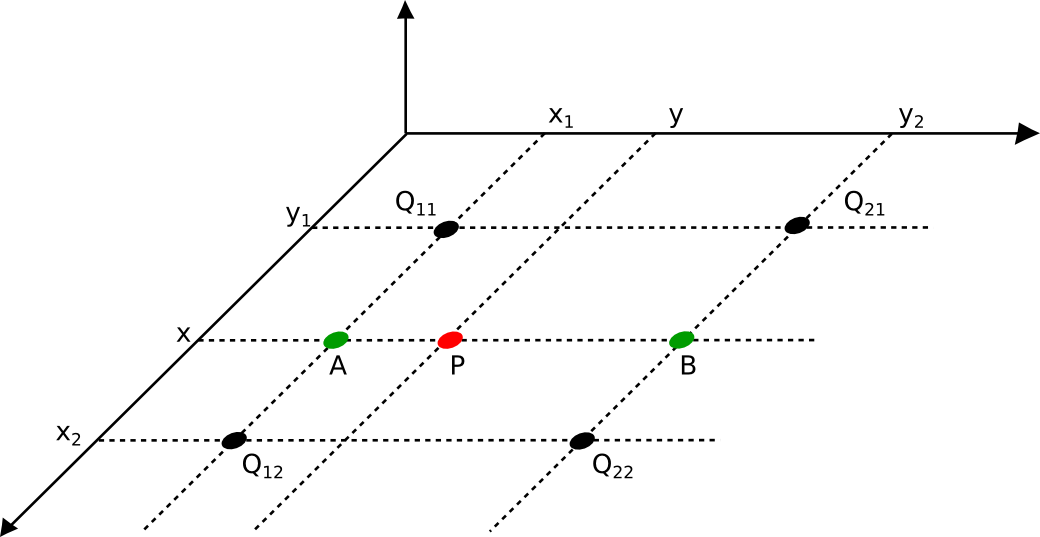
\includegraphics[width=0.65\textwidth]{./img/interpolace/bilinear.png}
    \caption[Bilinear interpol.]{\centering  Ilustrování principu bilineární interpoalce \footnotemark}
 \end{figure}   
\footnotetext{\url{http://postgis.net/docs/manual-2.1/}}



\paragraph{Bikubická spline} iterpolace je rozšíření kubické interpolace o druhý rozměr.; Principem je podobná bilineární interpolaci, s rozdílem, že k výpočtům odhadovaných bodu využívá kubické spline interpolace.  Využití \textit{spline} metody zajišťuje to, že první a druhá parciální derivace polynomu pro odhad koeficientů je spojitá. Oproti bilineární interpolaci je tak výsledný rastr vyhlazenější a celkový výsledek je přesnější. 



\paragraph*{Inverse Distance Weighting}
\acs{IDW} využívá k odhadu bodu \emph{P} základního statistického prvku. Určovaný bod \emph{P}  je počítán jako vážený průměr hodnot  bodů známých bodů $Q_{i}$.  Myšlenka je založena na předpokladu, že sobě bližší body jsou si hodnotou více podobné, než ty co jsou od sebe vzdálenější. Váhy se tedy počítají inverzně ze vzdáleností $d_{0,i}$. Pro nastavení citlivosti interpolace slouží parametr \emph{p}, který exponentem  vzdálenosti $d_{0,i}$. \cite{spatialinter}

\begin{equation}
P_{i}=\frac{\frac{1}{d_{0,i}^{p}}}{\sum_{i=1}^{n}\frac{1}{d_{0,i}^{p}}}
\end{equation}

Z tohoto vztahu plyne, že s rostoucím koeficientem \emph{p} mají jednotlivé  body $Q_{i}$ rozdílnější váhy. Při volbě $p=0$ se výsledný bod \emph{P} vypočte jako aritmetický průměr z všech bodů $Q_{i}$.

\paragraph*{Regularized spline with tension}























\newpage
\setcounter{footnote}{1}
\section{Časoprostorové analýzy}
Hlavní účelem GIS systému je  vytvoření informačního systému, který umožňuje získávání, ukládání, analýzu a vizualizaci dat, která mají prostorový rozsah povrchu Země. Všeobecně je hlavním cílem vytvoření operačních modelů založených na reálném světě. Pro modelování některých reálných jevů je nedílnou součástí časová složka. Z náhledu na historický vývoj většiny GIS software vyplývá, že primární zaměření vývoje bylo nejvíce zaměřeno na práci s prostorovými daty, nikoli však časoprostorovými. Software pro zpracování  časoprostorových dat byl z pravidla vyvíjen samostatně, mimo systémy GIS. Nicméně v poslední dekádě přestal být z velké části tento fakt pravdivý.\cite{geospatialanal} Systém GRASS nyní v nové verzi \textit{GRASS GIS 7 } obsahuje kompletně nově navržený balíček modulů TGRASS \footnote{\url{http://grass.osgeo.org/grass70/manuals/temporalintro.html}}, který integruje do tohoto GIS systému časový rozměr.

Hlavním cílem teoretické části je představení časoprostorových datových modelů s primárním zaměřením na model, který je implementován v  modulech TGRASS. S využitím TGRASS budou v praktické části definovány vhodné funkce pro analýzu zrekonstruovaných srážek pomocí vlastního modulu \textit{r.mwprecip}. K teoretické části byla jako primární zdroj využita kniha (\textit{Geographical information system vol.2})\cite{gistemporal}


\subsection{Terminologie}
V rámci této podkapitoly jsou čtenáři přiblíženy terminologické výrazy ohledně problematiky časoprostorových GIS. Hlavním zdrojem pro definice byla publikace \cite{pelekis}
\begin{description}
\item[Reprezentace času] Jednotlivé stavy geodat jsou odkazovány k  časovým okamžikům dvěma způsoby a to relativně  (\textit{dny,roky, minuty})  či absolutně (\textit{1990-30-06 1:35:59}). Možností relativní reprezentace je vyjádření času záporně (\textit{-rok}). Další reprezentace je vyjádřena pomocí klasického dělení časů (\textit {před- minulý, teď- současný, po- budoucí}).
\item[Diskrétně časový model] je takový model, kde se proměnné, tedy geodata  mění skokově. Geodata jednotlivých okamžiků na sebe navazují podle dostupného či zvoleného časového rozlišení. Vhodným příkladem je sčítání lidu v daném intervalu
\item[Kontinuální/spojitý časový model] je charakteristický jemným časovým rozlišením. Příkladem jsou geodata získaná ze seismografu, či kontinuálního měření průtoku řek.
\item[Časová topologie] je termín, který podstatou definice odpovídá  termínu prostorová topologie, s rozdílem že se jedná mimo prostorový rozměr i o časový. Časová topologie geodat definuje vztahy mezi jednotlivými okamžiky daných objektů v datasetu.
\item[Granularita] je ve spojení s časoprostorovými daty definován jako bod na dělené časové ose. Tento bod definuje počátek časové osy, která je dělena v daném rozlišení (zrnitosti). 
\end{description}

\subsection{Časoprostorové modely}

Časoprostorové modely se liší v jednotlivém pojetí vztahů, které propojují časovou složku s prostorovými daty. Současný vývoj a specifické nároky vědních oborů vytvořil poměrně velikou škálu časoprostorových modelů \cite{pelekis}, které jsou často sjednoceny  základní myšlenkou a liší se pouze specificky. Typicky jsou jednotlivé modely upravovány podle požadavků jejich  a  Níže jsou přiblíženy principy základních modelů se zaměřením na (Snapshot model), který je také časoprostorovým modelem  v TGRASS.

\subsubsection*{Snapshot model}
Jedná se o jeden z nejrozšířenějších a nejednodušších časoprostorových modelů. U tohoto modelu je začlenění časových složek aplikováno pomocí relačního modelu, který je charakteristický relačními tabulkami, tedy členění daných vektorových či rastrových rámců do jednotlivých časových vrstev/tabulek. Princip modelu je schématicky znázorněn na obrázku \ref{fig:snapshot}.

\begin{figure}[h!]
    \centering
    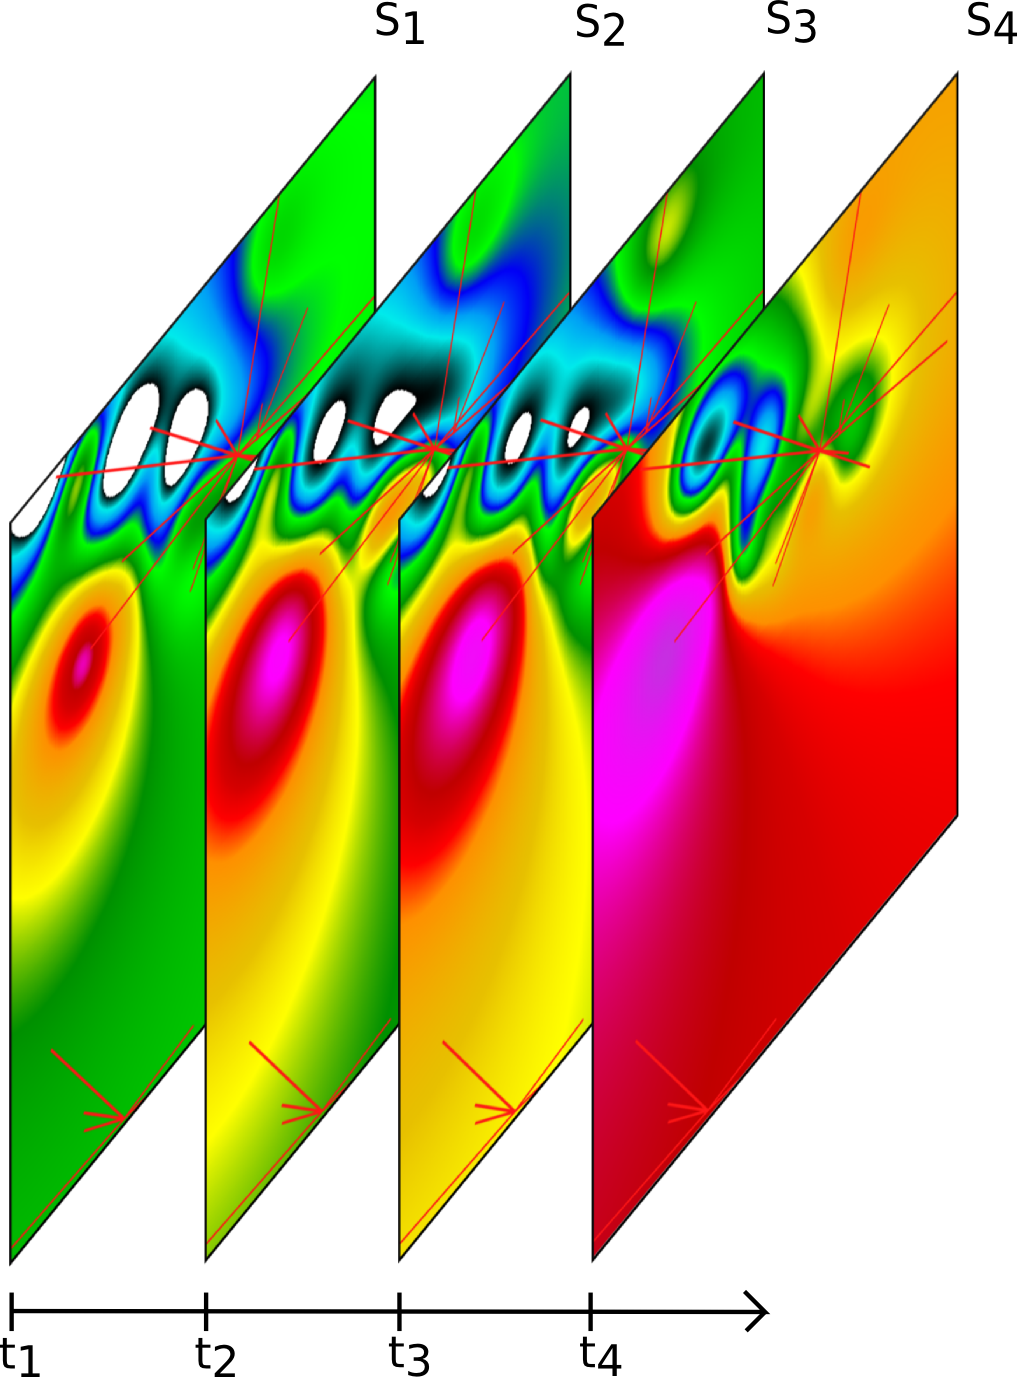
\includegraphics[width=0.4\textwidth]{./img/temporal/snapshot.png}
    \caption[Snapshot model]{Jednotlivé snímky \emph{S} reprezentují  geodata v čase \emph{t}. Obrázek schématicky znázorňuje vývoj dešťových srážek.  \centering \footnotemark }
        \label{fig:snapshot}
 \end{figure}   
\footnotetext{Podkladem pro obrázek byly využity výstupy z modulu r.mwprecip}

Tento model je specifický především pro rastrové interpretace. Hlavní výhoda  \textit{snapshot} modelu je v jednoduchosti a především vhodné struktury pro implementaci do GIS. Jak již bylo zmíněno, model uchovává jednotlivé vrstvy pro dané časové okamžiky odděleně, tedy jednotlivé tématické geoinformace zájmových oblastí jsou ukládány do separovaných vrstev.  Model  charakteristikou svého navržení odpovídá diskrétním systémům nikoli kontinuálním, tedy jednotlivé proměnné-geodata se mění v průběhu času skokově (nespojitě). Diskrétní modely jsou obecně vzato využívány v situacích, kdy je exaktní vyjádření velice obtížné a je výhodné problém reprezentovat zjednodušeně. Z toho mimo jiné pro GIS plyne, že jednotlivé snímky nemají informace o stavech  předchozího či následujícího časového okamžiku.
Nevýhodou tohoto modelu je datová redundance, která je způsobena ukládáním informací pro daný okamžik vždy v plném rozsahu.  Jednotlivá geodata jsou uchovávány pro časové okamžiky nenávazně na předchozích. Vezmeme-li pro názornost extrémní případ, kdy časový dataset obsahuje vrstvy znázorňující jev, který byl v průběhu času neměnný, tento model do úložiště počítače zapíše několikanásobně stejné geoinformace. Tato charakteristika je v GIS praxi poměrně nevýhodná, jelikož ve většině případů jsou změny mezi jednotlivými okamžiky malé.
Mezi nevýhody diskrétního modelování patří skoková interpretace problematiky. V GIS to má za důsledek to, že může nastat situace, kdy dojde mezi časovým krokem k velké změně, ta ovšem nebude zcela zaznamenána.
Pro srovnávání změn jednotlivých prostorových rámců v čase je díky architektuře modelu nutnost procházení a porovnávání buňky po buňce, či nastaveným kernelem, což vede k velké operační náročnosti.

\paragraph*{Time Composit}
Neboli \textit{\ac{STC}} byl navrhnut Lagran\cite{lagran} v letech 1988. Model \acs{STC} pracuje s vektorovou interpretací geodat.   Princip tohoto modelu spočívá v projekci linií do roviny, čímž se v průběhu času jednotlivé prostory v projekční rovině sjednotí a tím z nich vznikají polygony, síť. V databázi jsou pak pro jednotlivé polygony uchovávány atributy, které odpovídají jejich historii.
Model je charakteristický diskrétním systémem, kde jednotlivé časové skoky jsou relativní.

\paragraph*{Time-stamping model} 
Princip modelu je založen na dvojici časových razítek, které charakterizují čas vzniku a zániku, či současného stavu objektu. Časové razítko zániku objektu je definováno třemi stavy \texttt{now}, \texttt{currnetm}  a \texttt{null}. 
Síla tohoto modelu je při aplikacích, kde se jednotlivé objekty v průběhu dlouhé doby mění sporadicky. Model byl navržen a otestován na katastru nemovitostí, kde požadavky přesně odpovídají funkcím tohoto modelu.\cite{hunter}

\paragraph*{Event model}
Také \textit{Event-Oriented Model }, je blízký principu předchozího modelu. Model time-stamping nedokáže identifikovat jednotlivé změny v rámci datasetu. Oproti tomu je tento model rozšířený  o legovací soubor, do kterého jsou zaznamenávány jednotlivé časové instance objektů. Tento soubor představuje časovou topologii, která reprezentuje celou historii změn objektů, který je možné procházet a analyzovat.

\paragraph*{Object-Relationship}
jako jediný z výše zmíněných se tento model zaměřuje na vztahy a popis jednotlivých změn. O-R model je tedy čistě specifický dle zaměření dané problematiky. Specifikem  modelu je větší náročnost na definování jednotlivých vztahu mezi objekty než návrhem datové reprezentace. 

\paragraph*{Objektově orientovaný model}
\textit{Object-Oriented} model je principiálně podobný objektově orientovaným programovacím jazykům. Tato koncepce umožňuje vytvářet  objekty, třídy, metody, instance, dědičnost, operátory a dynamické vazby, tedy vše podstatné pro objektově orientovaný návrh. Díky tomu je možné poměrně uceleně simulovat reálné vztahy.  Jednotlivé objekty v průběhu času ukládají své entity, které tak tvoří historii instancí. Výhoda objektově orientovaného návrhu je v jednoduchém a intuitivním přístupu k jednotlivým informacím. 
















\chapter*{Praktická část}
\section{Rekonstrukce MV srážek v GRASS GIS}
\section{Modul r.mw.precip}

\subsection{Funkce}

\subsection{Použití}
\subsection{Implementace}

\subsubsection{}

\section{Modul v.link.precip}



\subsection{Modul r.mwprecip}
Nejdůležitější částí celé práce je navržení a implementace modulu, na jehož vstupu jsou hrubá data z MV vysílačů uložená v databázi PostgreSQL a výstupem jsou intenzity srážek pro jednotlivé MV spoje uložené v databázi. Systém GRASS GIS nativně podporuje databázi PostgreSQL s extenzí PostGIS. Funkcionalita modulu mimo spočtené intenzity srážek uložené v databázi, podporuje dvě základní reprezentace datových výstupů v GIS.  Výstupem modulu jsou jak plošně interpolované intenzity srážek v rastrové reprezentaci, tak i vektorová reprezentace srážkových intenzit pro jednotlivé MV spoje.
Mezi další podporu vstupních dat patří  načítání  dat ze srážkoměrů, které jsou výhodná k analýzám rekonstruovaných srážek z MV spojů.

\subsubsection{Vstup-data}   

\subsection{Výstup}





\section{Plošné interpolace srážek}


\section{Časoprostorové analýzy}


\subsubsection{Temporal GRASS GIS framework}
\subsubsection{Temporal GRASS GIS framework}


\subsection{Využitelnost}
\setcounter{footnote}{1}
\section{Závěr}
\section{Příloha}
\subsection{Dokumentace}
\subsection{Uživatelská příručka}




%\begin{enumerate*}
   % \item nastavit region na zvolenou rastrovou či vektorovou mapu
    %\item nastavit uložený region (\emph{named region})
   % \item nastavit aktuální výpočetní region
  %  \item zvolit souřadnice středu mapy a měřítko (nastavení regionu
 %   se automaticky vypočítá)
%\end{enumerate*}





\necislovana{Závěr}

Cílem této práce bylo 


\newpage
\necislovana{Seznam použitých zkratek}
\begin{acronym}[USA-CERL]
 	\acro{ANSI}{American National Standards Institute}
  	\acro{API}{Application Programming Interface}
  	\acro{DML}{Data Manipulate on Language}
  	\acro{DSD}{Drop size distribution}
  	\acro{DPZ}{Dálkový průzkum země}
  	\acro{DDL}{Data Definition Language}
  	\acro{EPSG}{Geodetic Parameter Set}	
  	
  	\acro{GIS}{Geographic Information System (Geografický informační systém)}
  	\acro{GNU GPL}{Všeobecná veřejná licence GNU (GNU General Public License)} 
	\acro{GRASS}{Geographical Resources Analysis Support System}
	\acro{GUI}{Graphical User Interface (Grafické uživatelské rozhraní)}
		
	
	\acro{HMM}{Hidden Markov Model} 
	\acro{IDW}{Inverse Distace Weighting} 
	\acro{IR}{Infra red (infračervené spektrum)} 
	
	\acro{ITU}{International Telecommunication Union}
	
	\acro{OGC}{Open Geospatial Consortium}
	\acro{OSGeo}{Open Source Geospatial Foundation} 
	\acro{ORDBMS}{objektově-relační atabázový systém}
	
  	\acro{RSL}{Received Signal Level}
  	\acro{STC}{The Space-Time Coposite Data Model}
    \acro{SRID}{Spatial Reference System Identifier}
	\acro{wxGUI}{WxPython-based GUI for GRASS}	
	
	\acro{WKT}{Well-known text}
\end{acronym}





\newpage
\renewcommand\baselinestretch{1.2}
\selectfont
\renewcommand{\refname}{Použité zdroje}
\phantomsection
\addcontentsline{toc}{section}{\refname}

\begin{thebibliography}{99}
\label{literatura}




\bibitem{radar_meterology}
RAGHAVAN, S. \textit {Radar meteorology}.
31 Oct 2003. Boston: Kluwer Academic Publishers, 2003, 549 s. ISBN 14-020-1604-2. 

\bibitem{flash_floods}
SENE, Kevin. \textit {Flash floods forecasting and warning}.
2013. Dordrecht: Springer, 2013. ISBN 978-940-0751-644. 

\bibitem{vanguard}
GREEN, McLaughlin a Milton LOMASK. \textit {Vanguard - A history: succes - AND AFTER http://history.nasa.gov/SP-4202/toc2.html}.
[online]. [cit. 2014-04-03]. URL:\textless\url {http://history.nasa.gov/SP-4202/chap12.html}

\bibitem{sejong}
STRANGEWAYS, Ian.  \textit {Precipitation: theory, measurement and distribution}.
New York: Cambridge University Press, 2007, x, 290 p. ISBN 978-052-1851-176. 

\bibitem{wmo}
World Meteorological Organization. \textit{Guide to meteorological instruments and methods of observation CHAPTER 6}. WMO-No. 8. Geneva, Switzerland: World Meteorological Organization, 2008. ISBN 978-926-3100-085. 

\bibitem{wren}
ASIT K. BISWAS {Notes and Records of the Royal Society of London: The Automatic Rain-Gauge of Sir Christopher Wren} UK: The Royal Society, 1967. ISSN 00359149. 

\bibitem{sevruk}
SEVRUK, B.\textit{Niederschlag als Wasserkreislauf-element. Theorie und Praxis der Niederschlagsmessung.} 
Zurich-Nitra: Eigenverlag ETH Zurich,  2004, 200 s, ISBN 80–969343–7–6.

\bibitem{chmu_navod}
Česká republika, \textit{Návod pro pozorovatele meteorologických stanic.}
In: Metodický předpis č. 13. Ostrava, 2013. URL:\textless\url {http://old.chmi.cz/OS/pdf/metodicky_navod/MP.pdf}


\bibitem{doppler}
DOVIAK, R. J.; D. S. Zrnic. \textit{Doppler Radar and Weather Observations (2nd ed.)}
(1993), San Diego CA: Academic Press, ISBN 0-12-221420-X.

\bibitem{kohout}
KOHOUT, Jan. \textit{Zpracování a prezentace srážkových dat měřících stanic meteorologického radaru pro ČHMÚ. Informační technologie pro praxi.}
Ostrava: TANGER, 2003. s. 101-103. ISBN 80-85988-90-9.

\bibitem{radar_chmu}
KRÁČMAR, Jan. Český hydrometeorologický ústav. \textit{Meteorologické radiolokátory.} ČHMÚ.
[online]. 1997-2011 [cit. 2014-04-06]. URL:\textless\url {http://portal.chmi.cz/files/portal/docs/meteo/rad/info_radar/index.html}

\bibitem{itu}
RECOMMENDATION ITU-R P.838-3. \textit{Specific attenuation model for rain for use in prediction methods}. 
ITU-R, (1992-1999-2003-2005). URL:\textless\url {https://www.itu.int/dms_pubrec/itu-r/rec/p/R-REC-P.838-3-200503-I!!PDF-E.pdf}

\bibitem{dsd}
CARLTON,W. Ulrich.\textit {Natural Variations in the Analytical Form of the Raindrop Size Distribution}. 
Department of Physics and Astronomy, Clemson University: Journal of Climate and Applied Meteorology, 1983, roč. 1983, č. 22. URL:\textless\url {http://radarmet.atmos.colostate.edu/AT741/papers/Ulbrich_DSD.pdf}

\bibitem{mv1}
ZINEVICH, A., H. MESSER a P. ALPERT. \textit {Prediction of rainfall intensity measurement errors using commercial microwave communication links}. Atmospheric Measurement Techniques [online]. 2010, vol. 3, issue 5, s. 1385-1402 [cit. 2014-04-13]. DOI: 10.5194/amt-3-1385-2010. URL:\textless\url { http://www.atmos-meas-tech.net/3/1385/2010/}

\bibitem{mv2}
MESSER, H. \textit {Environmental Monitoring by Wireless Communication Networks.}, Science [online]. 2006-05-05, vol. 312, issue 5774, s. 713-713 [cit. 2014-04-14]. DOI: 10.1126/science.1120034. URL:\textless\url {http://www.sciencemag.org/cgi/doi/10.1126/science.1120034}

\bibitem{wetat}
M, Schleiss, Rieckermann J. a Berne A.  \textit{Quantification and Modeling of Wet-Antenna Attenuation for Commercial Microwave Links}[online]. 06 únor 2013. Geoscience and Remote Sensing Letters, IEEE, 2013[cit. 2014-04-13]. Volume:10. 

\bibitem{countryw}
OVEREEM, Aart, Hidde LEIJNSE a Remko UIJLENHOET.  \textit{Country-wide rainfall maps from cellular communication networks} [online]. 2012 [cit. 2014-04-13]. 110: 8. DOI: 10.1073/pnas.121796111. URL:\textless\url {http://www.pnas.org/content/110/8/2741.full}

\bibitem{radiolinks}
LEIJNSE, H., R. UIJLENHOET a J. N. M. STRICKER. \textit{Rainfall measurement using radio links from cellular communication networks.} Water Resources Research [online]. 2007, vol. 43, issue 3, n/a-n/a [cit. 2014-04-13]. DOI: 10.1029/2006WR005631. URL:\textless\url {http://doi.wiley.com/10.1029/2006WR005631}

\bibitem{comparsinmv}
Asaf Rayitsfeld, Rana Samuels, Artem Zinevich, Uri Hadar, Pinhas Alpert, \textit{Comparison of two methodologies for long term rainfall monitoring using a commercial microwave communication system}. Atmospheric Research, Volumes 104–105, February 2012, Pages 119-127, ISSN 0169-8095, http://dx.doi.org/10.1016/j.atmosres.2011.08.011.
URL:\textless\url {http://www.sciencedirect.com/science/article/pii/S0169809511002626}

\bibitem{grasshist}
Historical Notes. \textit{GRASS GIS} [online]. 1998-2014 [cit. 2014-04-17]. URL:\textless\url {http://grass.osgeo.org/home/history/}

\bibitem{geospatialanal}
SMITH, Michael J, Michael F GOODCHILD a Paul LONGLEY. \textit{Geospatial analysis: a comprehensive guide to principles, techniques and software tools} [online]. 4th ed. Winchelsea, UK: The Winchelsea Press, c2013, s. 130-135 [cit. 2014-04-18]. ISBN 9781906221980.

\bibitem{gistemporal}
LONGLEY, Paul.\textit{Geographical information systems: principles, techniques, management, and applications}[online]. 2nd ed., abridged. Hoboken, N.J.: John Wiley, c2005., ch 8, [cit. 2014-04-18]. ISBN 0471735450.

\bibitem{lagran}
G. Langran and N.R. Chrisman. \textit{A framework for temporal geographic infor-
mation}. In: Cartographica: The International Journal for Geographic Infor-
mation and Geovisualization 25.3 (1988), pp. 1–14.

\bibitem{hunter}
J. HUNTER, Gary a Ian P. WILLIAMSON. \textit{Journal of Geographic Information System} The Development of a Historical Digital Cadastral Database. 1990, no.2, s. 167-179. URL:\textless\url {http://csdila.unimelb.edu.au/publication/journals/ipw_90_historicalDCDB.pdf}


\bibitem{pelekis}
PELEKIS, Nikos, Babis THEODOULIDIS, Ioannis KOPANAKIS a Yannis THEODORIDIS. Literature Review of Spatio-Temporal Database Models. \textit{The Knowledge Engineering Review}. 2004, September 2004, č. 19, s. 235-274. 

\bibitem{sql1999}
ISO/IEC 9075-2:1999. \textit{Information technology: Database languages SQL}. Part 2: Foundation. SQL/Foundation, 2011. 

\bibitem{postgre}
CHEN, Hao, Heechul HEECHUL a Jin XIAO. \textit{Concept Architecture of PostgreSQL}. 2009. \textit{http://www.inf.fu-berlin.de/lehre/WS09/DBS-Tech/Material/ConceptArchPostres.pdf}

\bibitem{bares}
BARĚŠ, Pavel. \textit{Implementace materializovaných pohled; v PostgreSQL}. Praha, 2010. Bakalářská práce. ČVUT FIT. Vedoucí práce Ing. Zdeněk Kotala.

\bibitem{sqlmm}
STOLZE, Knut. \textit{SQL/MM Spatial: The Standard to Manage Spatial Data in Relational Database Systems. 2003.}\textless\url {http://doesen0.informatik.uni-leipzig.de/proceedings/paper/68.pdf}



\bibitem{postgis}
CHRISTL, Arnulf.\textit{Introduction to Spatial Data Management with Postgis }
[online]. [cit. 2014-04-20].\textless\url { http://www.mapbender.org/presentations/Spatial_Data_Management_Arnulf_Christl/Spatial_Data_Management_Arnulf_Christl.pdf}


\bibitem{spatialinter}
Mitas, L., Mitasova, H.,\textit{Geographical Information Systems}
2002; Burrough and McDonnell; Bonham-Carter, 1996 \textless\url {http://csiss.org/learning_resources/content/good_sa/#Interpolation}

\bibitem{ }
\textit{ }
\textless\url {  }

\bibitem{ }
\textit{ }
\textless\url {  }

\bibitem{ }
\textit{ }
\textless\url {  }

\bibitem{ }
\textit{ }
\textless\url {  }

\bibitem{ }
\textit{ }
\textless\url {  }

\bibitem{ }
\textit{ }
\textless\url {  }

\bibitem{ }
\textit{ }
\textless\url {  }

\bibitem{ }
\textit{ }
\textless\url {  }

\bibitem{ }
\textit{ }
\textless\url {  }

\bibitem{ }
\textit{ }
\textless\url {  }

\bibitem{ }
\textit{ }
\textless\url {  }


\bibitem{ }
\textit{ }
\textless\url {  }





\end{thebibliography}
\end{document}



